% design.tex -- the final report on the multi-cycle RV32I SoC for the Digilent Genesys 2.
%
% Build: make (in this directory) -> build/design.pdf, two pdflatex passes, from the
% committed figures; no Vivado or board needed. make figures regenerates the scriptable
% figures; figures/README.md lists every figure and how it is made.
%
% Source material: notes.md in this directory holds the design rationale behind each
% module (bugs, workarounds, timing subtleties, deliberate quirks), grouped by module
% and naming the signal each note concerns.
% Read the matching section of notes.md before writing each chapter below, and cite it
% instead of repeating it. The current RTL (rtl/), the firmware (fw/), the simulation
% harness (sim/) and the baseline numbers (docs/baseline.md) are the other inputs.
%
% Each chapter not yet written holds one \planned note: what the chapter will hold.
% Figures go in figures/ and are included with \includegraphics{figures/<name>}.

\pdfminorversion=7  % the figures are PDF 1.7
\documentclass[11pt,a4paper]{report}

\usepackage[utf8]{inputenc}
\usepackage[T1]{fontenc}
\usepackage{lmodern}
\usepackage[margin=2.5cm]{geometry}
\usepackage{graphicx}
\usepackage{subcaption}
\usepackage{booktabs}
\usepackage{xcolor}
\usepackage{titlesec}
\usepackage{tikz}
\usetikzlibrary{arrows.meta,positioning}
\usepackage{animate}
\usepackage[hidelinks]{hyperref}
\usepackage{qrcode}

% Callouts on board photos: a label in the margin, an arrow with a white halo, so that it
% shows on the black board and on the white page alike.
\tikzset{
  callout/.style={-{Stealth[length=2.2mm]}, line width=0.8pt, draw=red!80!black,
    preaction={draw=white, line width=2.4pt, -{Stealth[length=2.8mm]}}},
  callout label/.style={font=\footnotesize, text width=3cm, inner sep=1pt},
}

% The report's module colours, the same as in scripts/gui_helper.tcl and figures/README.md.
\definecolor{modcore}{RGB}{0,114,178}
\definecolor{modregfile}{RGB}{86,180,233}
\definecolor{modram}{RGB}{230,159,0}
\definecolor{modbus}{RGB}{240,228,66}
\definecolor{moduart}{RGB}{0,158,115}
\definecolor{modflash}{RGB}{204,121,167}
\definecolor{modclock}{RGB}{153,153,153}
\newcommand{\swatch}[1]{{\setlength{\fboxsep}{0pt}\fcolorbox{gray}{#1}{\rule{0pt}{1.6ex}\rule{1.6em}{0pt}}}}

% Compact chapter headings: about 25 pages of body in 13 chapters.
\titleformat{\chapter}{\normalfont\LARGE\bfseries}{\thechapter}{1em}{}
\titlespacing*{\chapter}{0pt}{0pt}{2ex}

% Two figures may share the top of a page with a few lines of text, instead of a float page
% of their own and the lines on the next page.
\renewcommand{\topfraction}{0.9}
\renewcommand{\textfraction}{0.07}
\renewcommand{\floatpagefraction}{0.85}

% What a chapter will hold, until it is written.
\newcommand{\planned}[1]{\noindent{\color{gray}\itshape To hold: #1}\par}

% A citation of the design notes, docs/design/notes.md, by section heading: the notes hold
% the full reasoning, the report states the choice.
\newcommand{\notes}[1]{(\texttt{notes.md}, ``#1'')}

\title{A Multi-cycle RV32I System on Chip for the Digilent Genesys 2}
\author{Amit Malach \\ Supervisor: Prof.\ Avi Mendelson \\ Technion -- Israel Institute of Technology}
\date{\today}

\begin{document}

% The title page and the first contents page are both page 1: no anchor for the title page.
\hypersetup{pageanchor=false}
\maketitle
\hypersetup{pageanchor=true}
\tableofcontents

\chapter{Introduction}
\planned{what the system is and why it was built, the opening figure of the board, and the
acknowledgement of Bruno Levy's \emph{From Blinker to RISC-V}~\cite{levy-learnfpga}.}

\chapter{Board and tools}
\planned{the Genesys~2 parts the design touches, with cited excerpts of Digilent's
schematic~\cite{digilent-genesys2-rm}, the I/O package view, and the tool versions.}

% The top view, figures/board.jpg, is the title page's photo. The callouts below point in the
% photo's pixels, measured on a 1400-pixel-wide copy: one unit is 9.2 cm / 1400.
\begin{figure}[htbp]
  \centering
  \begin{tikzpicture}[x=9.2cm/1400, y=-9.2cm/1400]
    \node[anchor=north west, inner sep=0] at (0,0)
      {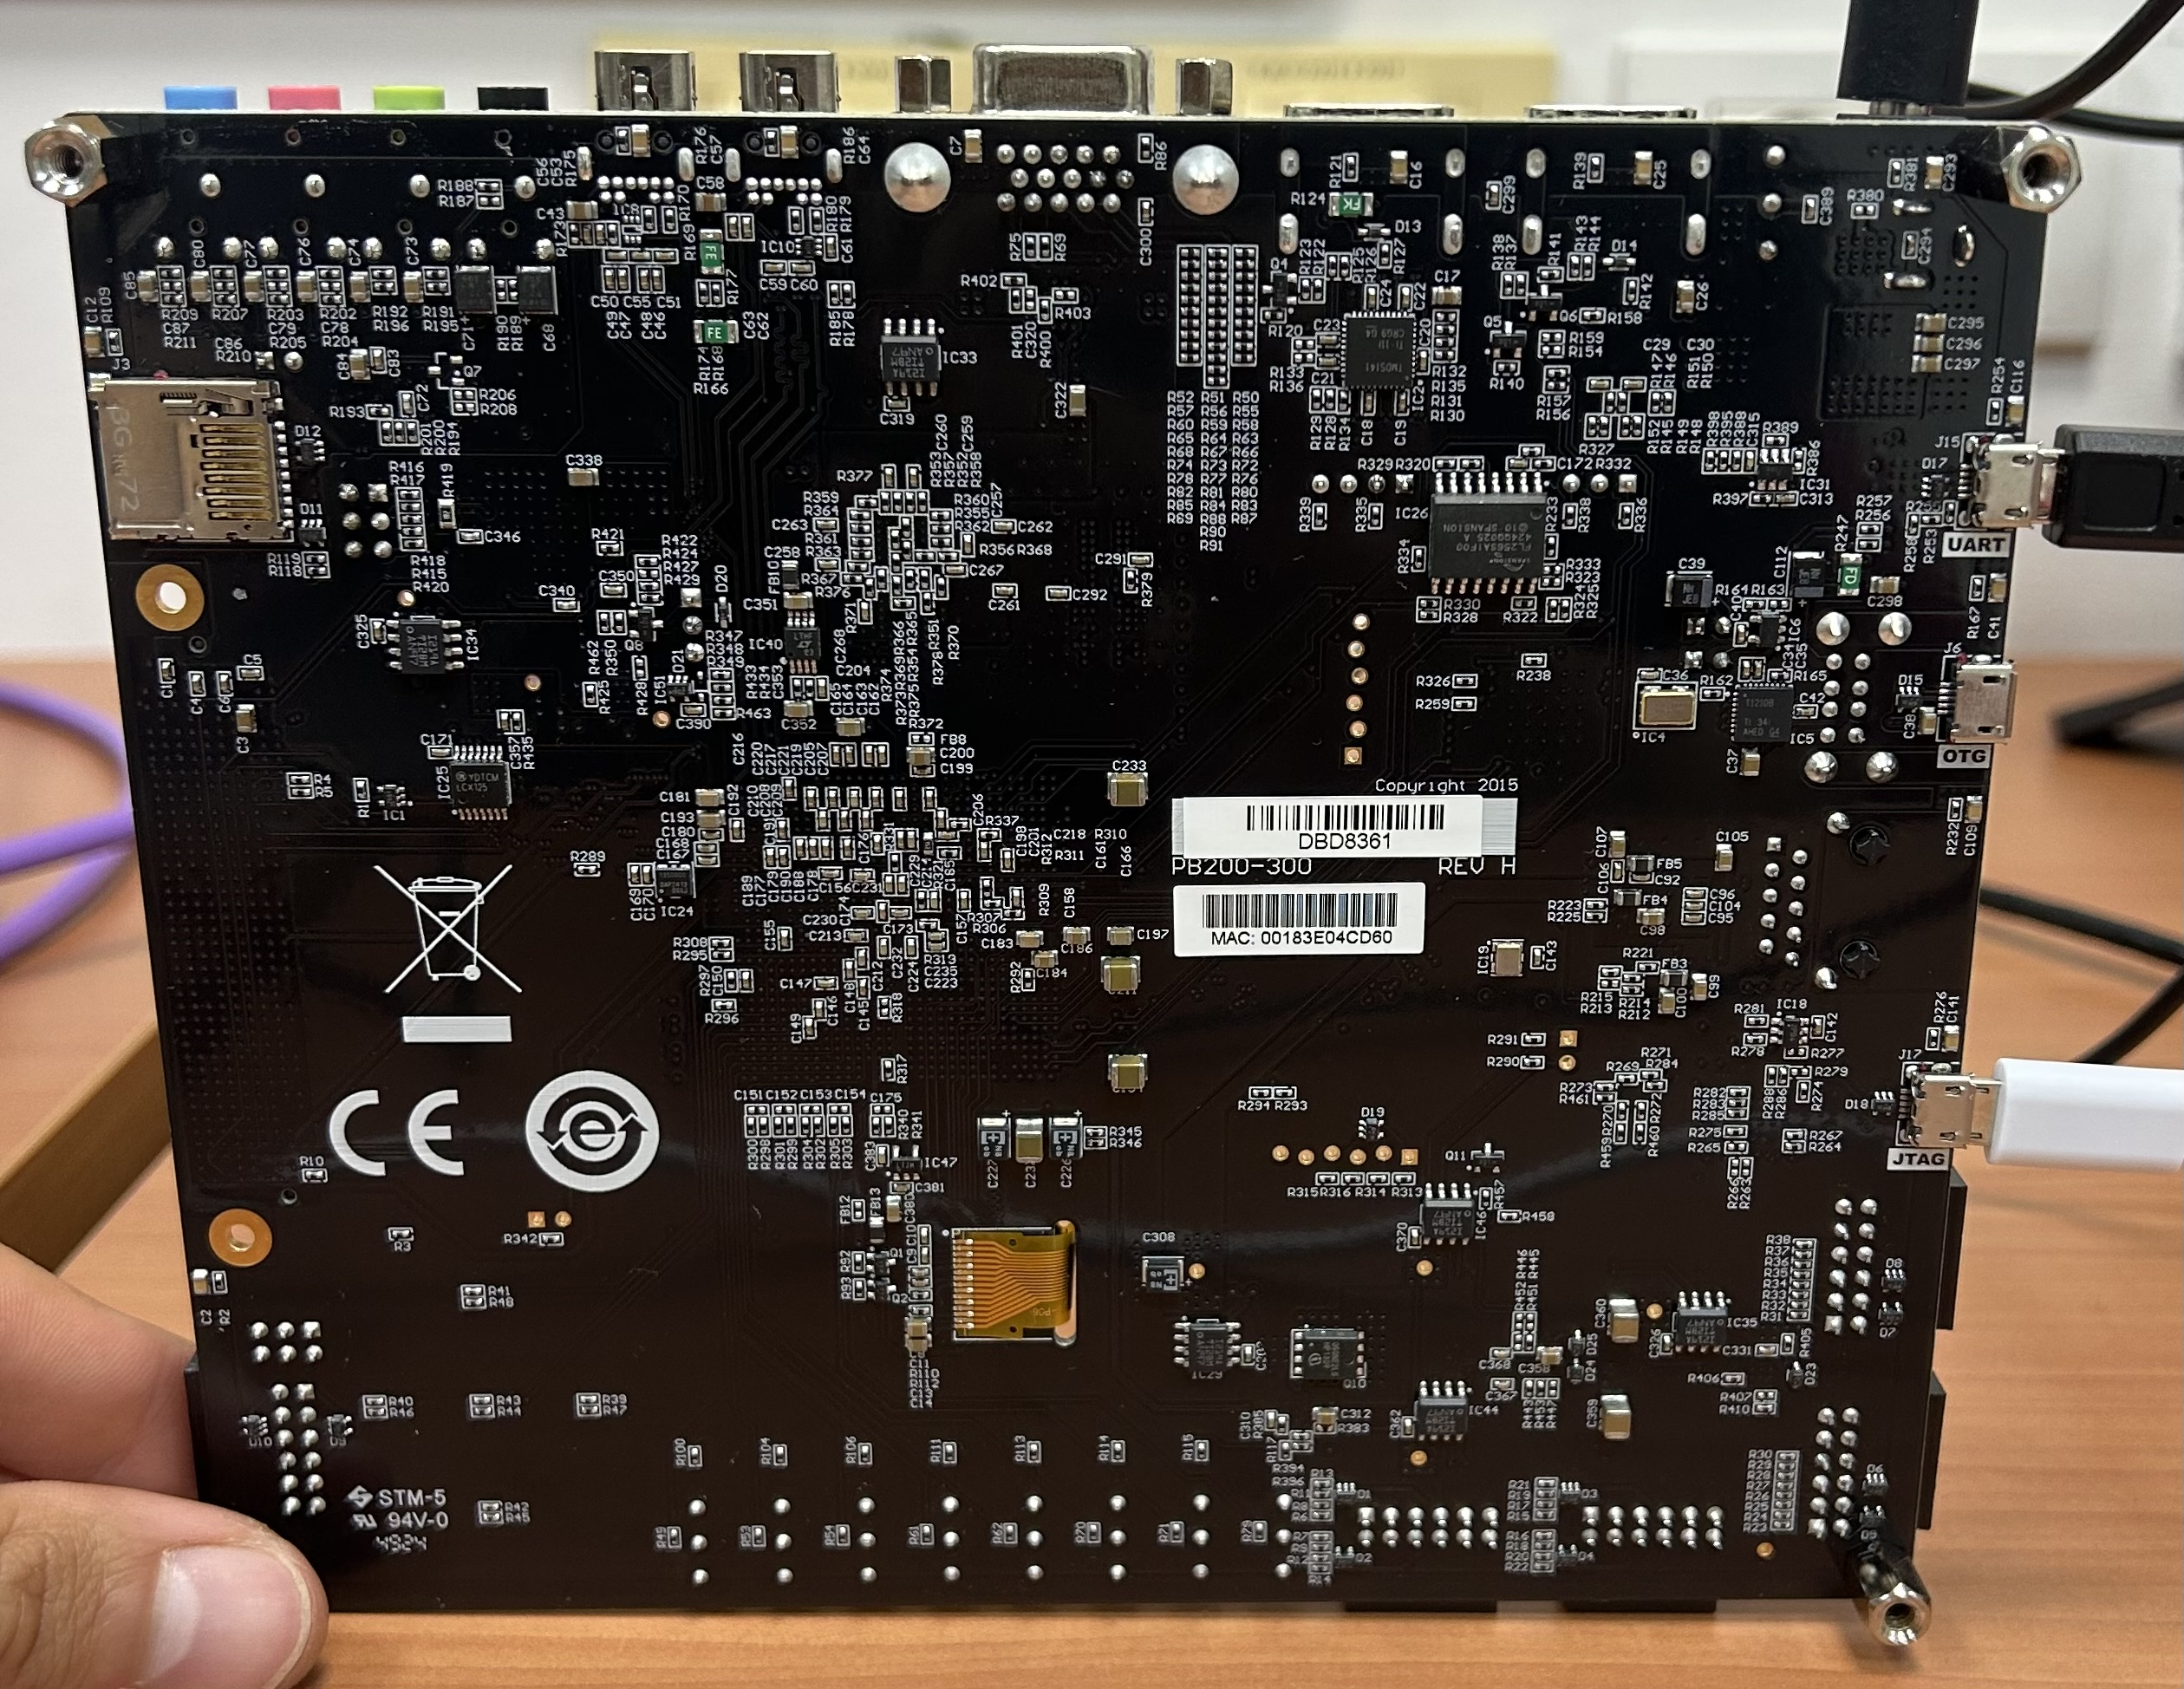
\includegraphics[width=9.2cm]{figures/board_bottom}};
    % Left margin, top to bottom.
    \node[callout label, anchor=east, align=flush right] (sd) at (-40,250)
      {microSD slot (J3)};
    \node[callout label, anchor=east, align=flush right] (ina) at (-40,410)
      {INA219 current\\monitors};
    \node[callout label, anchor=east, align=flush right] (dec) at (-40,570)
      {FPGA decoupling\\capacitors};
    \node[callout label, anchor=east, align=flush right] (pcb) at (-40,730)
      {board PB200-300,\\revision~H};
    \node[callout label, anchor=east, align=flush right] (oled) at (-40,890)
      {OLED display's\\flex cable};
    % Right margin, top to bottom.
    \node[callout label, anchor=west, align=flush left] (tmds) at (1440,120)
      {HDMI buffer,\\TMDS141};
    \node[callout label, anchor=west, align=flush left] (uart) at (1440,270)
      {\textbf{UART} micro-USB\\port (J15)};
    \node[callout label, anchor=west, align=flush left] (qspi) at (1440,420)
      {\textbf{QSPI flash},\\S25FL256S (IC26)};
    \node[callout label, anchor=west, align=flush left] (otg) at (1440,610)
      {USB OTG port (J6),\\TUSB1210 PHY (IC5)};
    \node[callout label, anchor=west, align=flush left] (jtag) at (1440,800)
      {\textbf{JTAG} micro-USB\\port (J17)};
    \draw[callout] (sd.east) -- (122,293);
    \draw[callout] (ina.east) -- (271,414);
    \draw[callout] (ina.east) -- (584,231);
    \draw[callout] (dec.east) -- (560,470);
    \draw[callout] (pcb.east) -- (800,553);
    \draw[callout] (oled.east) -- (645,820);
    \draw[callout] (tmds.west) -- (885,225);
    \draw[callout] (uart.west) -- (1285,310);
    \draw[callout] (qspi.west) -- (953,343);
    \draw[callout] (otg.west) -- (1265,452);
    \draw[callout] (otg.west) -- (1130,458);
    \draw[callout] (jtag.west) -- (1255,700);
  \end{tikzpicture}
  \caption{The underside of the Genesys~2, the top view mirrored: the UART and JTAG ports,
    on the left edge from above, are on the right here. Bold labels name the parts this design
    uses: the QSPI flash, which holds the bitstream, the demo data and the flash-boot program
    (Chapter~\ref{ch:flash}), and the two micro-USB ports that carry its UART output and its
    programming. The parts are named from their markings and Digilent's
    schematic~\cite{digilent-genesys2-sch}.}
  \label{fig:board-bottom}
\end{figure}

\begin{table}[htbp]
  \centering
  \begin{tabular}{@{}cll@{}}
    \toprule
    Colour & Module & Its ports \\
    \midrule
    \swatch{modcore} & the core: \texttt{Processor}, \texttt{Decoder}, \texttt{Control},
      \texttt{ALU} & \\
    \swatch{modregfile} & \texttt{RegisterFile} & \\
    \swatch{modram} & \texttt{Memory}, the RAM & \\
    \swatch{modbus} & \texttt{IOBus}, the LED register & \texttt{LEDS} \\
    \swatch{moduart} & \texttt{UartTx} & \texttt{uart\_rx\_out}, \texttt{uart\_tx\_in} \\
    \swatch{modflash} & \texttt{SPIFlash}, with \texttt{STARTUPE2} & \texttt{spiflash\_*} \\
    \swatch{modclock} & clock and reset & \texttt{sysclk\_*}, \texttt{RESET} \\
    \swatch{white} & the worst setup path, selected & \\
    \bottomrule
  \end{tabular}
  \caption{The module colours of every Vivado view in this report: Okabe-Ito colours, which
    stay distinct under the common forms of colour blindness. A selected path shows in
    Vivado's selection white.}
  \label{tab:module-colours}
\end{table}

\begin{figure}[htbp]
  \centering
  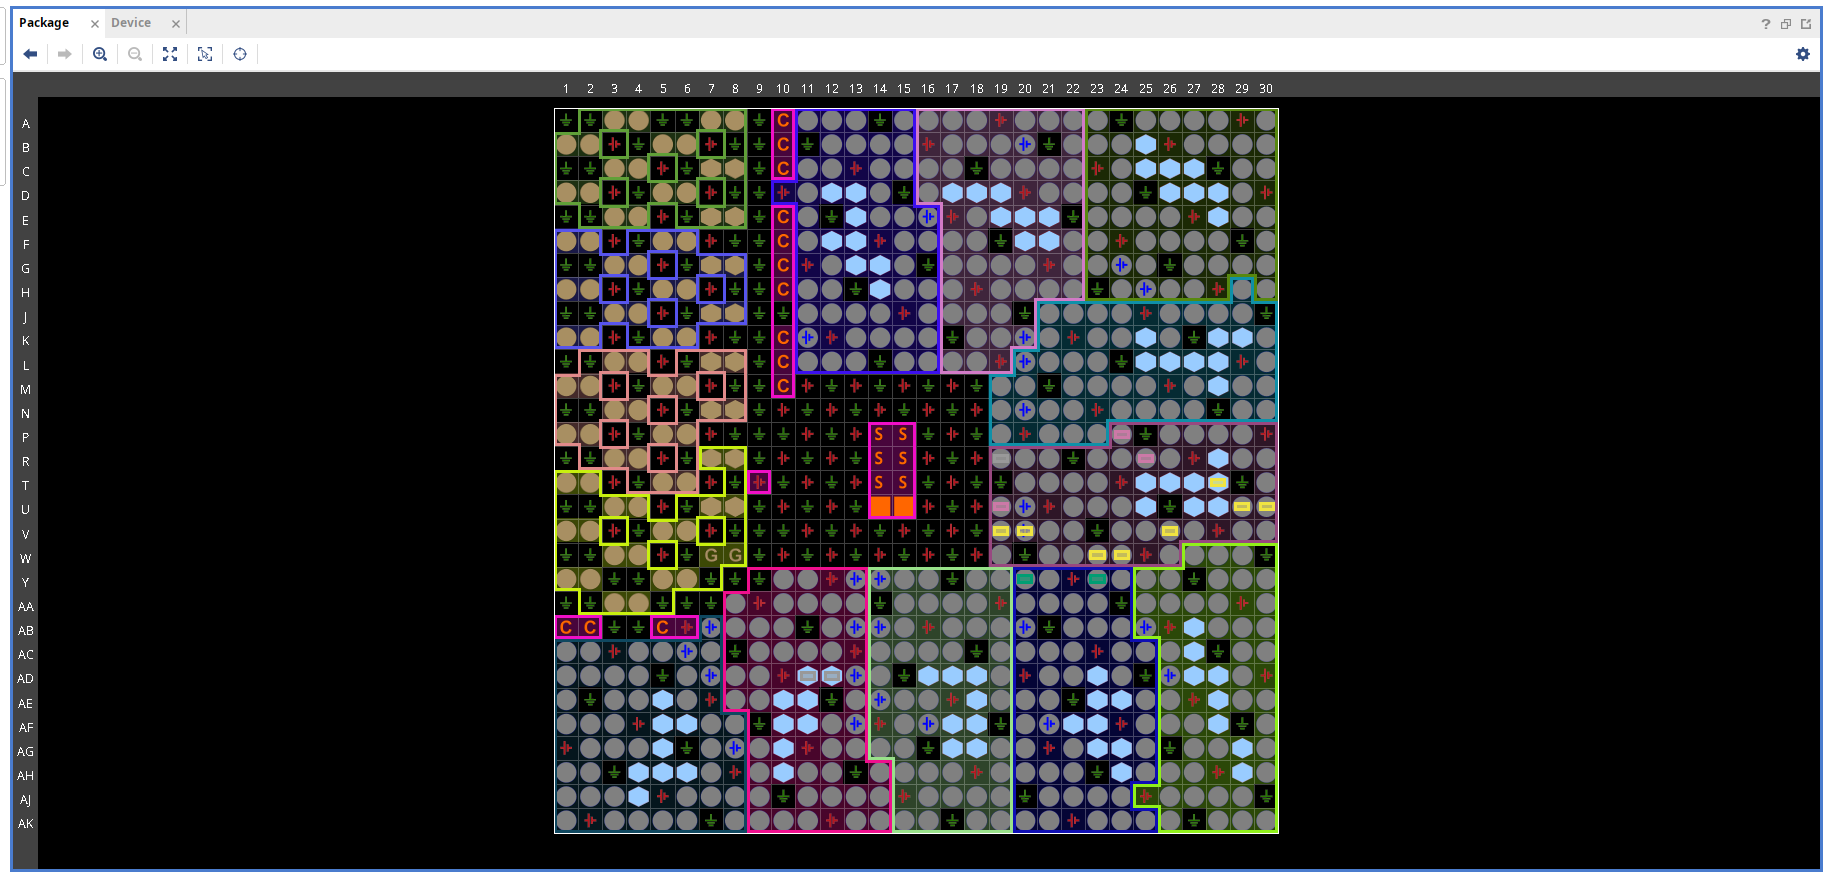
\includegraphics[width=\textwidth]{figures/vivado_io_package}
  \caption{Vivado's Package view of the FFG900 package (Layout $>$ I/O Planning), rows A to
    AK and columns 1 to 30, from the routed design. The design's 16 ports show in their
    modules' colours (Table~\ref{tab:module-colours}): the eight LEDs, the three flash pins,
    the two UART pins, the reset button and the differential system clock. Fifteen of them
    are bonded IOBs; \texttt{uart\_tx\_in}, on Y20, has no load and so no IOB, but keeps its
    pin.}
  \label{fig:io-package}
\end{figure}

\chapter{Repository tour}
\planned{one table of folders and one of make entry points.}

\chapter{System architecture}
\label{ch:arch}

The SoC is six modules in one clock domain, wired together by \texttt{SOC}, the top level
(Figure~\ref{fig:soc}), with four more inside the core. The core sees one bus; everything else
hangs off that bus.
This chapter gives the bus and the modules, the memory map and its decode, and the clock and
reset. Each section names the design-notes section that holds the full reasoning.

\begin{figure}[htbp]
  \centering
  \begin{subfigure}{\textwidth}
    \centering
    \resizebox{\textwidth}{!}{%
    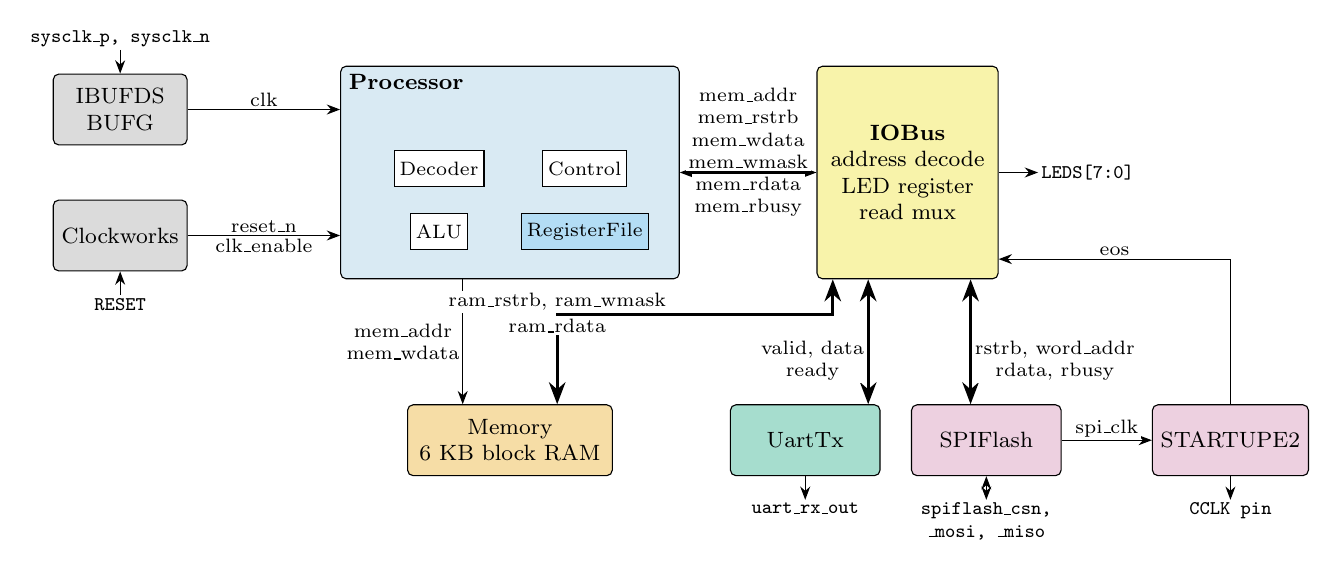
\begin{tikzpicture}[x=1cm, y=1cm, font=\footnotesize, >=Stealth,
        block/.style={draw, rounded corners=2pt, minimum height=0.9cm, align=center,
          inner sep=3pt},
        sub/.style={draw, fill=white, font=\scriptsize, inner sep=2pt, minimum height=0.45cm},
        port/.style={font=\scriptsize\ttfamily, inner sep=1pt, align=center},
        wire/.style={font=\scriptsize, inner sep=1pt, fill=white, align=center},
        bus/.style={<->, line width=1.1pt},
        sig/.style={->}]
      % clock and reset, the left column, with the board's pins above and below
      \node[block, fill=modclock!35, minimum width=1.7cm] (clk) at (0,2.1) {IBUFDS\\BUFG};
      \node[block, fill=modclock!35, minimum width=1.7cm] (cw) at (0,0.5) {Clockworks};
      \node[port, above=0.3cm of clk] (sysclk) {sysclk\_p, sysclk\_n};
      \node[port, below=0.3cm of cw] (rst) {RESET};
      \draw[sig] (sysclk) -- (clk);
      \draw[sig] (rst) -- (cw);
      % the core
      \node[block, fill=modcore!15, minimum width=4.3cm, minimum height=2.7cm] (cpu)
        at (4.95,1.3) {};
      \node[anchor=north west, font=\footnotesize\bfseries, inner sep=3pt] at (cpu.north west)
        {Processor};
      \node[sub] (dec) at (4.05,1.35) {Decoder};
      \node[sub] (ctl) at (5.9,1.35) {Control};
      \node[sub] (alu) at (4.05,0.55) {ALU};
      \node[sub, fill=modregfile!45] (rf) at (5.9,0.55) {RegisterFile};
      \draw[sig] (clk.east) -- node[wire, above] {clk} (cpu.west |- clk.east);
      \draw[sig] (cw.east) -- node[wire, above] {reset\_n} node[wire, below] {clk\_enable}
        (cpu.west |- cw.east);
      % the bus
      \node[block, fill=modbus!45, minimum width=2.3cm, minimum height=2.7cm] (bus)
        at (10,1.3) {\textbf{IOBus}\\address decode\\LED register\\read mux};
      \draw[bus] (cpu.east |- bus.west) -- node[wire, above]
        {mem\_addr\\mem\_rstrb\\mem\_wdata\\mem\_wmask} node[wire, below]
        {mem\_rdata\\mem\_rbusy} (bus.west);
      \node[port, right=0.5cm of bus] (leds) {LEDS[7:0]};
      \draw[sig] (bus) -- (leds);
      % memory and peripherals, the bottom row
      \node[block, fill=modram!35, minimum width=2.6cm] (ram) at (4.95,-2.1)
        {Memory\\6 KB block RAM};
      \node[block, fill=moduart!35, minimum width=1.9cm] (uart) at (8.7,-2.1) {UartTx};
      \node[block, fill=modflash!35, minimum width=1.9cm] (flash) at (11,-2.1) {SPIFlash};
      \node[block, fill=modflash!35, minimum width=1.8cm] (su) at (14.1,-2.1) {STARTUPE2};
      \draw[sig] (cpu.south -| 4.35,0) -- node[wire, left] {mem\_addr\\mem\_wdata}
        (ram.north -| 4.35,0);
      \draw[bus] (bus.south -| 9.05,0) -- ++(0,-0.45) -| node[wire, above, pos=0.5]
        {ram\_rstrb, ram\_wmask} node[wire, below, pos=0.5] {ram\_rdata}
        (ram.north -| 5.55,0);
      \draw[bus] (bus.south -| 9.5,0) -- node[wire, left, pos=0.65] {valid, data\\ready}
        (uart.north -| 9.5,0);
      \draw[bus] (bus.south -| 10.8,0) -- node[wire, right, pos=0.65]
        {rstrb, word\_addr\\rdata, rbusy} (flash.north -| 10.8,0);
      \draw[sig] (flash.east) -- node[wire, above] {spi\_clk} (su.west);
      \draw[sig] (su.north) |- node[wire, above, pos=0.75] {eos} (bus.east |- 0,0.2);
      \node[port, below=0.3cm of uart] (txpin) {uart\_rx\_out};
      \draw[sig] (uart) -- (txpin);
      \node[port, below=0.3cm of flash] (fpins) {spiflash\_csn,\\\_mosi, \_miso};
      \draw[<->] (flash) -- (fpins);
      \node[port, below=0.3cm of su] (cclk) {CCLK pin};
      \draw[sig] (su) -- (cclk);
    \end{tikzpicture}}
    \caption{The block diagram, from \texttt{rtl/SOC.v}, in the module colours of
      Table~\ref{tab:module-colours}. The thick arrows are the core's bus and the handshakes
      \texttt{IOBus} derives from it. \texttt{clk}, 200~MHz, reaches every block;
      \texttt{reset\_n} and \texttt{clk\_enable}, drawn into the core only, also reach
      \texttt{IOBus}, the RAM (\texttt{clk\_enable}) and the UART (\texttt{reset\_n}).}
    \label{fig:soc-block}
  \end{subfigure}
  \par\bigskip
  \begin{subfigure}{\textwidth}
    \centering
    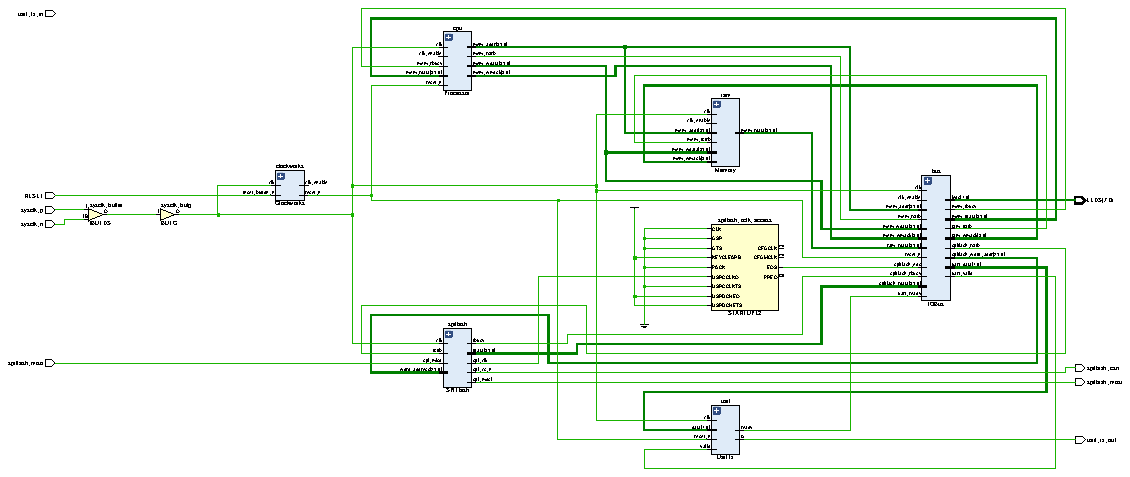
\includegraphics[width=0.9\textwidth]{figures/rtl_soc}
    \caption{Vivado's RTL schematic of the same top level, elaborated from the Verilog with
      \texttt{synth\_design -rtl}: the six instances under their names in \texttt{SOC.v},
      and the three primitives, \texttt{IBUFDS} and \texttt{BUFG} on the clock and
      \texttt{STARTUPE2} on the flash clock.}
    \label{fig:rtl-soc}
  \end{subfigure}
  \caption{The SoC as drawn and as Vivado inferred it.}
  \label{fig:soc}
\end{figure}

\section{The bus and the modules}

The core, \texttt{Processor}, sees one bus and nothing else: a 32-bit byte address, a
one-cycle read strobe, 32 bits of read data, 32 bits of write data with a four-bit byte
mask, and a busy input. The bus has no acknowledge. A read requested with
\texttt{mem\_rstrb} is answered on \texttt{mem\_rdata} in the next cycle, unless
\texttt{mem\_rbusy} is high, and a write lands on the edge where \texttt{mem\_wmask} is
non-zero. Every address falls in some region, so no access is refused
\notes{Processor bus has no notion of RAM versus device}.

Everything around the core follows from that contract. \texttt{IOBus} decodes the address
into three regions, forwards the strobe and the mask to the RAM, holds the LED register,
turns a store into the UART's send pulse and a flash read into an SPI transaction, and
multiplexes the read data back. \texttt{Memory} is 6~KB of block RAM with one port, shared
by instruction fetch and by loads and stores: there is no separate instruction memory. Its
read is registered, which is why the core waits a cycle after every read, and its write
lands on the same edge, which is why a store needs no wait
\notes{Read and write timing are not symmetric}. \texttt{UartTx} sends 8N1 at 115\,200~baud
and \texttt{SPIFlash} reads one 32-bit word per transaction, at a sixth of the system
clock. The flash controller is the only block that stalls the core, by holding
\texttt{mem\_rbusy} for the length of a transaction; the RAM and the IO registers always
answer in the next cycle \notes{Only flash reads stall the core; read mux}.
Chapters~\ref{ch:memio} and~\ref{ch:flash} give each module's timing.
Figure~\ref{fig:rtl-soc} is what Vivado makes of \texttt{SOC.v} before synthesis: the same
six instances. \texttt{Clockworks} is among them but contributes no cell to the netlist,
as Section~\ref{sec:clock} explains.

\section{Memory map and address decode}
\label{sec:memmap}

Table~\ref{tab:memory-map} is the memory map, defined once in \texttt{rtl/defines.vh}. The
firmware carries copies of its values in \texttt{fw/io.h} and the start-up code, and a lint
rule holds every copy equal to the defines (Chapter~\ref{ch:verif}).

\begin{table}[htbp]
  \centering
  \small
  \begin{tabular}{@{}llp{5.5cm}l@{}}
    \toprule
    Byte address & Selected by & Region or register & Access \\
    \midrule
    \texttt{0x0000\_0000}--\texttt{0x0000\_17FF} & no region bit & RAM, 6~KB (1536 words)
      & read, write, fetch \\
    \texttt{0x0040\_0000} & bit 22 & \texttt{IO\_BASE}, the IO registers & \\
    \quad\texttt{+ 0x04} & bit 2 & \texttt{IO\_LEDS}, the LED register & write \\
    \quad\texttt{+ 0x08} & bit 3 & \texttt{IO\_UART\_DAT}, send one byte & write \\
    \quad\texttt{+ 0x10} & bit 4 & \texttt{IO\_UART\_CNTL}, status; bit 9 = busy & read \\
    \texttt{0x0100\_0000}--\texttt{0x01FF\_FFFF} & bit 24 & SPI flash, a 16~MB window on
      the chip & read, fetch \\
    \quad\texttt{0x01D0\_0000}--\texttt{0x01FF\_FFFF} & & the code window, 3~MB, where
      flash boot starts & \\
    \bottomrule
  \end{tabular}
  \caption{The memory map (\texttt{rtl/defines.vh}). The reset vector is
    \texttt{0x0000\_0000} in BRAM boot and \texttt{0x01D0\_0000} in flash boot
    (Chapter~\ref{ch:flash}).}
  \label{tab:memory-map}
\end{table}

A region is chosen by one address bit, not by a comparator: bit~24 selects the flash, bit~22
selects the IO registers when bit~24 is clear, and an address with neither bit set is RAM.
Inside the IO region each register owns one bit as well, bits~2, 3 and~4, so a store to
\texttt{IO\_BASE + 4} lights the LEDs and a store to \texttt{IO\_BASE + 8} sends a byte. The
whole decode is a few bit tests in \texttt{IOBus}, the address masked with a base and
OR-reduced, and a register is as cheap as a region \notes{Address decode: one bit per
region, one-hot IO registers, why bit 24}.

The flash bit is the one that was chosen with care, because it fixes how much of the chip
is reachable: everything below the selector bit is the offset inside the flash. Bit~23 would
leave 8~MB, which does not reach past the 10.9~MB bitstream that sits at the start of the
same chip; bit~24 leaves 24 bits, 16~MB, exactly the three address bytes of the flash's
\texttt{03h} read command. The IO bit only has to lie between the RAM and the flash, and
bit~22 does. The code window at 13~MB, and why, are in Chapter~\ref{ch:flash}.

The decode has three consequences worth knowing before writing firmware. Nothing is
rejected: an address with no region bit selects the RAM, past its 6~KB end as well, and what
such an access does is undefined; in simulation it reads \texttt{x}. Only the UART
status register answers a read; the LED and UART data registers, and any other IO address,
read as zero. And a write to flash space does nothing: the controller only reads. To add a
peripheral, give it the next free bit of the IO word address, bit~5 at byte offset
\texttt{0x20}, decode it in \texttt{IOBus} as the three existing ones are decoded, add it to
the read mux if it answers reads, and add its copy in \texttt{fw/io.h} to the lint rule.

\section{Clock and reset}
\label{sec:clock}

The board's 200~MHz oscillator drives a differential pair, so the clock enters through
\texttt{IBUFDS}, which turns the pair into one signal, and \texttt{BUFG}, which puts it on a
global clock net \notes{Genesys 2 differential clock input}. That net, \texttt{clk}, is the
only clock in the design; its 5~ns period is the one timing constraint, met with 0.219~ns to
spare (Chapter~\ref{ch:results}).

\texttt{Clockworks} derives two signals from the clock and the button. \texttt{clk\_enable}
is a gearbox: with the parameter \texttt{SLOW} set to $n$, it is high for one cycle in
$2^n$, and the core, the bus and the RAM advance only on those cycles, while the UART and
the flash controller run every cycle, so the baud rate and the SPI clock stay right
\notes{Gearbox counter}. With \texttt{SLOW} at 20 the core runs a million times slower and
the LEDs can be watched; the shipped design sets it to~0, \texttt{clk\_enable} is the
constant~1, and the module synthesises to nothing.

\texttt{reset\_n} is the CPU RESET button, active-low on this board, forwarded as it is: no
synchroniser and no debounce. Every reset in the design is synchronous, and three places
have one: the core's \texttt{pc}, \texttt{instr} and FSM state, the LED register, and the
UART's transmitter. The register file, the RAM and the flash controller have none; the
register file because the core fetches an instruction before it reads any register. The
core's and the LED register's resets are not gated by \texttt{clk\_enable}, so a slowed
design still resets on the next edge \notes{Synchronous reset and the clock enable}.
The core's three registers also declare their reset value as their initial value, which is
what configuration loads into the flip-flop on a 7-series part, so the core leaves
configuration already in its reset state and starts without a press of the button
\notes{Power-on state matches the reset state}. The LED register and the UART declare
none and configure to zero: the LEDs dark, and the UART in its idle state, whose first
clock raises the line and \texttt{ready}. In flash boot a press is still needed on the
board, for a reason that lies in the flash controller's start-up, not here
(Chapter~\ref{ch:board}).

The one subtlety of the reset is where the FSM lands. Reset puts the core in
\texttt{WAIT\_DATA}, not \texttt{FETCH\_INSTR}, because \texttt{FETCH\_INSTR} asserts the
read strobe for as long as it lasts, and a reset held for many cycles with \texttt{pc} in
flash space would restart the SPI transaction on every cycle with chip select held low.
\texttt{WAIT\_DATA} asserts nothing, and falls through to \texttt{FETCH\_INSTR} in the first
cycle after the button is released: one cycle at boot buys a correctly framed first
transaction \notes{Reset lands in WAIT\_DATA, not FETCH\_INSTR}.

\chapter{The multi-cycle core}
\label{ch:core}

\texttt{Processor} executes RV32I, the base integer instruction set, and nothing beyond it:
no M extension, no interrupts, no control and status registers; \texttt{ECALL} and
\texttt{EBREAK} stop the core (Appendix~\ref{app:isa}). It is a multi-cycle core: one
instruction at a time, several clock cycles each, one FSM state per cycle. \texttt{Control}
is the FSM; \texttt{Decoder}, \texttt{ALU} and \texttt{RegisterFile} are what their names
say; \texttt{Processor} holds \texttt{pc}, the instruction register and the glue between
the other four.

\section{The state machine}

\begin{figure}[htbp]
  \centering
  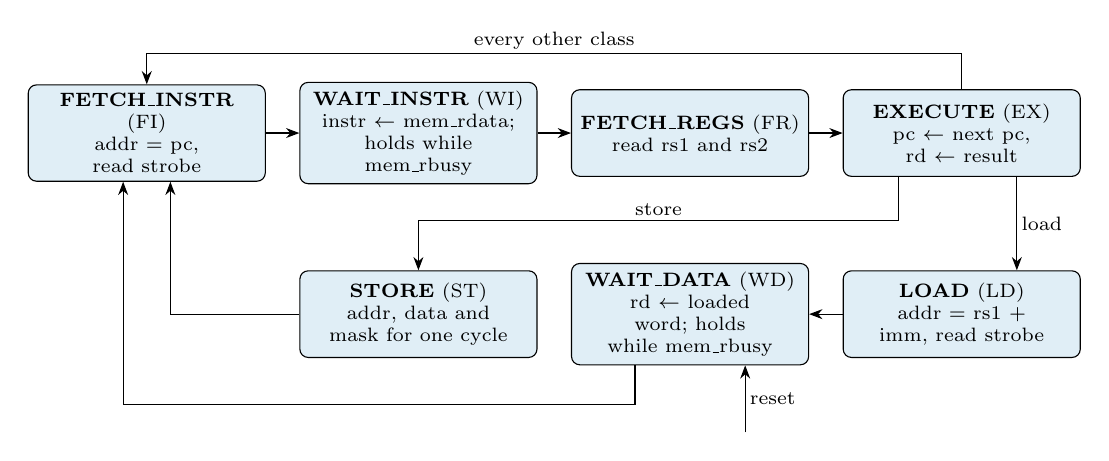
\begin{tikzpicture}[x=1cm, y=1cm, >=Stealth, font=\scriptsize,
      state/.style={draw, rounded corners=3pt, fill=modcore!12, text width=2.8cm,
        minimum height=1.1cm, align=center, inner sep=3pt},
      lbl/.style={fill=white, inner sep=1.5pt}]
    \node[state] (fi) at (0,0) {\textbf{FETCH\_INSTR} (FI)\\addr $=$ pc, read strobe};
    \node[state] (wi) at (3.45,0) {\textbf{WAIT\_INSTR} (WI)\\instr $\leftarrow$ mem\_rdata;
      holds while mem\_rbusy};
    \node[state] (fr) at (6.9,0) {\textbf{FETCH\_REGS} (FR)\\read rs1 and rs2};
    \node[state] (ex) at (10.35,0) {\textbf{EXECUTE} (EX)\\pc $\leftarrow$ next pc,
      rd $\leftarrow$ result};
    \node[state] (ld) at (10.35,-2.3) {\textbf{LOAD} (LD)\\addr $=$ rs1 $+$ imm, read strobe};
    \node[state] (wd) at (6.9,-2.3) {\textbf{WAIT\_DATA} (WD)\\rd $\leftarrow$ loaded word;
      holds while mem\_rbusy};
    \node[state] (st) at (3.45,-2.3) {\textbf{STORE} (ST)\\addr, data and mask for one
      cycle};
    \draw[->] (fi) -- (wi);
    \draw[->] (wi) -- (fr);
    \draw[->] (fr) -- (ex);
    \draw[->] (ex.north) -- ++(0,0.45) -| node[lbl, pos=0.25, above] {every other class}
      (fi.north);
    \draw[->] ([xshift=7mm]ex.south) -- node[lbl, right] {load} ([xshift=7mm]ld.north);
    \draw[->] ([xshift=-8mm]ex.south) -- ++(0,-0.55) -| node[lbl, pos=0.25, above] {store}
      (st.north);
    \draw[->] (ld) -- (wd);
    \draw[->] ([xshift=-7mm]wd.south) -- ++(0,-0.5) -| ([xshift=-3mm]fi.south);
    \draw[->] (st.west) -| ([xshift=3mm]fi.south);
    \draw[->] ([xshift=7mm, yshift=-0.85cm]wd.south) -- node[lbl, right] {reset}
      ([xshift=7mm]wd.south);
  \end{tikzpicture}
  \caption{The control FSM of \texttt{rtl/Control.v}: seven states, one cycle each, except
    the two waits, which hold while the flash controller is busy. The two-letter codes are
    the ones Figure~\ref{fig:wave-fsm} uses.}
  \label{fig:fsm}
\end{figure}

An instruction takes several cycles because the RAM answers a read one cycle after it is
requested, and because the register file's read is synchronous too, so each of those
needs its own state \notes{Why one instruction takes several cycles}.
Figure~\ref{fig:fsm} shows the seven. \texttt{FETCH\_INSTR} drives \texttt{pc} on the bus
with the read strobe; \texttt{WAIT\_INSTR} latches the word the RAM returns;
\texttt{FETCH\_REGS} latches \texttt{rs1} and \texttt{rs2}; \texttt{EXECUTE} loads
\texttt{pc} with its next value and writes \texttt{rd} for every instruction but a load, a
store or a branch. A load goes on to \texttt{LOAD}, which drives the data address with the
strobe, and \texttt{WAIT\_DATA}, which writes the returned word to \texttt{rd}. A store goes
to \texttt{STORE}, which drives the address, the data and the byte mask for one cycle; the
RAM writes on that same edge, so there is no wait after a store \notes{STORE needs no wait
state}. The two waits are the only states that can last longer than a cycle: they hold
while \texttt{mem\_rbusy} is high, which only the flash controller raises
\notes{Instruction fetch stalls on mem\_rbusy}.

\texttt{Control} decodes four one-cycle strobes from the state, \texttt{latch\_instr},
\texttt{read\_regs}, \texttt{update\_pc} and \texttt{write\_rd}, already qualified with
\texttt{clk\_enable} and \texttt{reset\_n}, so each datapath register tests only its
strobe. \texttt{write\_rd} in \texttt{WAIT\_DATA} is gated by \texttt{mem\_rbusy} as well,
or a stalled flash load would write the bus's garbage to \texttt{rd} on every stalled cycle
\notes{Write-back enable gated by mem\_rbusy in WAIT\_DATA}. Table~\ref{tab:cycles} gives
the cost per instruction class.

\begin{table}[htbp]
  \centering
  \begin{tabular}{@{}p{6.4cm}lc@{}}
    \toprule
    Instruction class & States & Cycles \\
    \midrule
    ALU, register and immediate; LUI, AUIPC; JAL, JALR; branch & FI WI FR EX & 4 \\
    Load: LB, LH, LW, LBU, LHU & FI WI FR EX LD WD & 6 \\
    Store: SB, SH, SW & FI WI FR EX ST & 5 \\
    SYSTEM: ECALL, EBREAK & FI WI FR EX, \texttt{pc} unchanged & 4, repeated \\
    \bottomrule
  \end{tabular}
  \caption{Cycles per instruction class from the RAM. A SYSTEM instruction leaves
    \texttt{pc} alone, so the core fetches it again, forever. Every instruction fetched from
    the flash, and every load from it, adds the SPI transaction to its wait state
    (Chapter~\ref{ch:memio}).}
  \label{tab:cycles}
\end{table}

Two of the four cycles of the commonest class are the fetch. A pipelined core would
overlap the fetch of one instruction with the execution of the last and retire close to one
instruction per cycle: a gain of four to six on code bound by computation. The demos of
Chapter~\ref{ch:board} are bound by the UART, which sets their pace at any clock, so for
them the multi-cycle core costs nothing visible. Pipelining is the first extension in
Chapter~\ref{ch:next}.

\section{The datapath}

\texttt{Decoder} is purely combinational on the instruction register: the ten class flags
from the opcode, disjoint, so at most one is high and exactly one for every instruction the
core implements; the register indices and
the \texttt{funct3} and \texttt{funct7} fields, at fixed positions in every format; and the
five immediates, sign-extended from bit~31. It also settles the two meanings of
\texttt{funct7[5]}: a subtraction only in the register form, since there is no
\texttt{SUBI} and an \texttt{ADDI} whose immediate happens to set bit~30 must still add,
and an arithmetic shift in both forms \notes{ADD versus SUB: funct7[5] alone is not
enough}.

\texttt{RegisterFile} is the 32 integer registers, in LUT RAM: a synchronous read of
\texttt{rs1} and \texttt{rs2} on \texttt{read\_regs}, a synchronous write of \texttt{rd} on
\texttt{write\_rd}, and \texttt{x0} never written and read as zero explicitly
\notes{x0 reads as zero explicitly}. \texttt{ALU} is combinational
(Figure~\ref{fig:rtl-alu}): its second operand is \texttt{rs2} for register instructions and
the I-immediate for everything else, the shift amount is the low five bits of that operand
either way, \texttt{funct3} picks one of the eight operations, and a second case on
\texttt{funct3} computes the six branch conditions on \texttt{rs1} and \texttt{rs2}, with a
default of zero so that no latch is inferred \notes{Branch comparator default arm}. Both
arms of the right shift are signed: with one of them unsigned, Verilog's \texttt{>>>} shifts
logically, and \texttt{SRA} behaved as \texttt{SRL} until the golden trace caught it
(Chapters~\ref{ch:verif} and~\ref{ch:next}).

\begin{figure}[tbp]
  \centering
  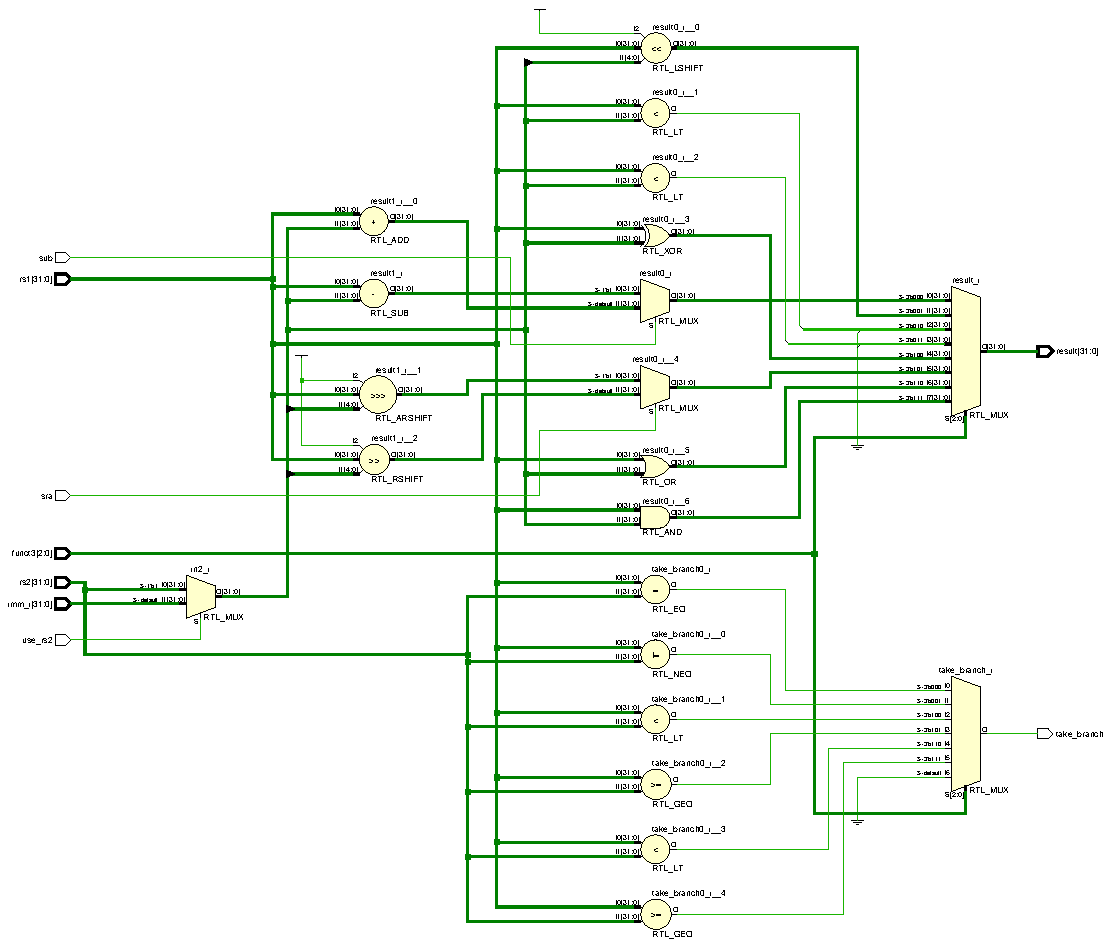
\includegraphics[width=0.5\textwidth]{figures/rtl_alu}
  \caption{Vivado's RTL schematic of \texttt{rtl/ALU.v}, elaborated as its own top so that
    its ports frame the drawing. Upper half: the operand multiplexer on the left, then the
    adder and subtractor, the shifters, the comparators and the logic operations, into the
    result multiplexer on the right. Lower half: the branch comparators, into the
    multiplexer that yields \texttt{take\_branch}. After synthesis nearly all of this merges
    into the LUTs around the register file (Chapter~\ref{ch:results}).}
  \label{fig:rtl-alu}
\end{figure}

The rest of \texttt{Processor} is the glue between these. A multiplexer chooses the next
\texttt{pc}: the branch target when a branch is taken, the jump target for \texttt{JAL},
\texttt{rs1} plus the immediate with bit~0 cleared for \texttt{JALR}, otherwise
\texttt{pc + 4} \notes{Why jalr\_target is a named wire}. An adder forms the load or store
address from \texttt{rs1} and the I- or S-immediate. The memory moves whole words, so a byte
or halfword load picks its lane by the address's low two bits and sign-extends unless
\texttt{funct3[2]} says not to, and a store broadcasts \texttt{rs2} into every lane it could
land in and lets the byte mask select \notes{Store data is broadcast to every lane; the
mask selects}. The write-back multiplexer gives \texttt{rd} its value: \texttt{pc + 4} for
the jumps, the U-immediate for \texttt{LUI}, \texttt{pc} plus it for \texttt{AUIPC}, the
aligned load data, or the ALU result. The worst timing path of the design runs through
this glue, from the instruction register through the decoder and the ALU's carry chain to
the register file's write port (Chapter~\ref{ch:results}).

\section{One instruction through the states}

Figure~\ref{fig:wave-fsm} is the simulated core at the end of \texttt{main}'s prologue in
the mandelbrot demo, where the frame counter, just stored to the stack, is loaded back and
written to the LEDs: four instructions, 19 cycles, every state of Figure~\ref{fig:fsm}.

\begin{figure}[tbp]
  \centering
  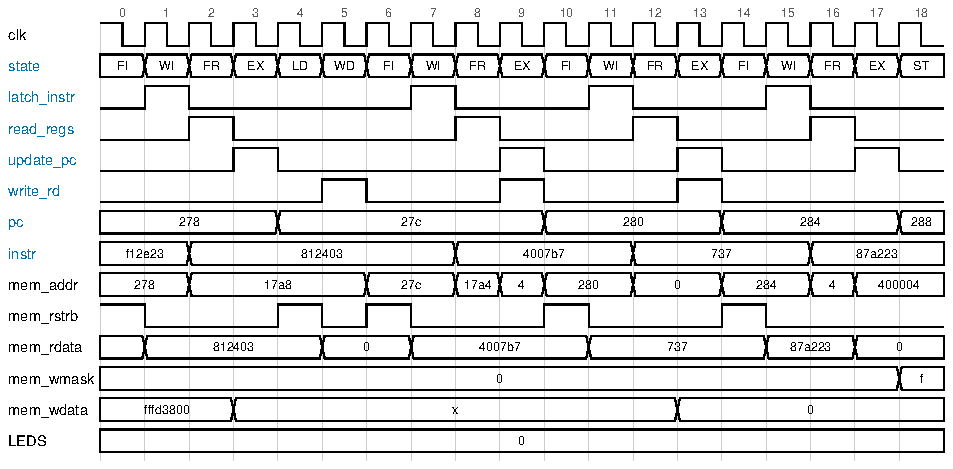
\includegraphics[width=0.88\textwidth]{figures/wave_fsm}
  \caption{Four instructions of the mandelbrot demo in the simulated SoC, from the VCD of
    \texttt{docs/design/scripts/waves/WaveBench.v}: \texttt{lw s0,8(sp)} at \texttt{0x278},
    \texttt{lui a5,0x400}, \texttt{lui a4,0x0} and \texttt{sw s0,4(a5)}, the store to the
    LED register. The core's signals are in blue, the bus in black; bus values are in hex
    with leading zeros dropped, and a value is left blank where it does not fit its cycle.
    \texttt{mem\_wdata} reads \texttt{x} while the instruction's \texttt{rs2} field names
    a register no instruction has written yet: the register file has no reset.}
  \label{fig:wave-fsm}
\end{figure}

The load takes cycles 0 to~5. In \texttt{FETCH\_INSTR} the bus address is \texttt{pc},
\texttt{0x278}, with the strobe; in \texttt{WAIT\_INSTR} the RAM answers with the
instruction word, \texttt{0x00812403}, and \texttt{latch\_instr} moves it into
\texttt{instr} on the edge that ends the cycle. From then on the bus address is the
load-store address, \texttt{sp + 8}. \texttt{EXECUTE} advances \texttt{pc} to
\texttt{0x27c}; \texttt{LOAD} asserts the strobe at the data address; \texttt{WAIT\_DATA}
sees the word,~0, and \texttt{write\_rd} writes it to \texttt{s0}. The two \texttt{LUI}s
take four cycles each, cycles 6 to~13, writing \texttt{rd} in \texttt{EXECUTE}. The store,
cycles 14 to~18, writes no register, so \texttt{write\_rd} stays low in its
\texttt{EXECUTE}; in \texttt{STORE} the bus carries the LED register's address,
\texttt{0x400004}, the byte mask \texttt{f} and the data, and the register takes the value
on the edge that ends the window. Each read is answered one cycle after its strobe, and no
cycle is spent on the store: the two facts about the memory that shaped the FSM.

\chapter{Memory and memory-mapped IO}
\label{ch:memio}
\planned{the RAM's read and write timing, the LED register, the UART data and status
registers, and a simulated waveform of a flash read stalling the core.}

\chapter{Boot modes and the SPI flash}
\label{ch:flash}
\planned{BRAM boot against flash boot, the flash layout, the STARTUPE2 route to the flash
clock pin~\cite{ug470}, and execute-in-place.}

\chapter{From C to the board}
\planned{the mandelbrot demo from C source to UART output, with a real excerpt at each stage,
and the flash-boot branch of the flow.}

\chapter{Verification}
\label{ch:verif}
\planned{the ALU unit bench, the golden trace, the regression and the gates.}

\chapter{Implementation results}
\label{ch:results}
\planned{per-module utilization, the timing result and the worst path, the device views, a
logic-level or slack chart, and the power breakdown.}

\begin{figure}[htbp]
  \centering
  \begin{subfigure}[t]{0.49\textwidth}
    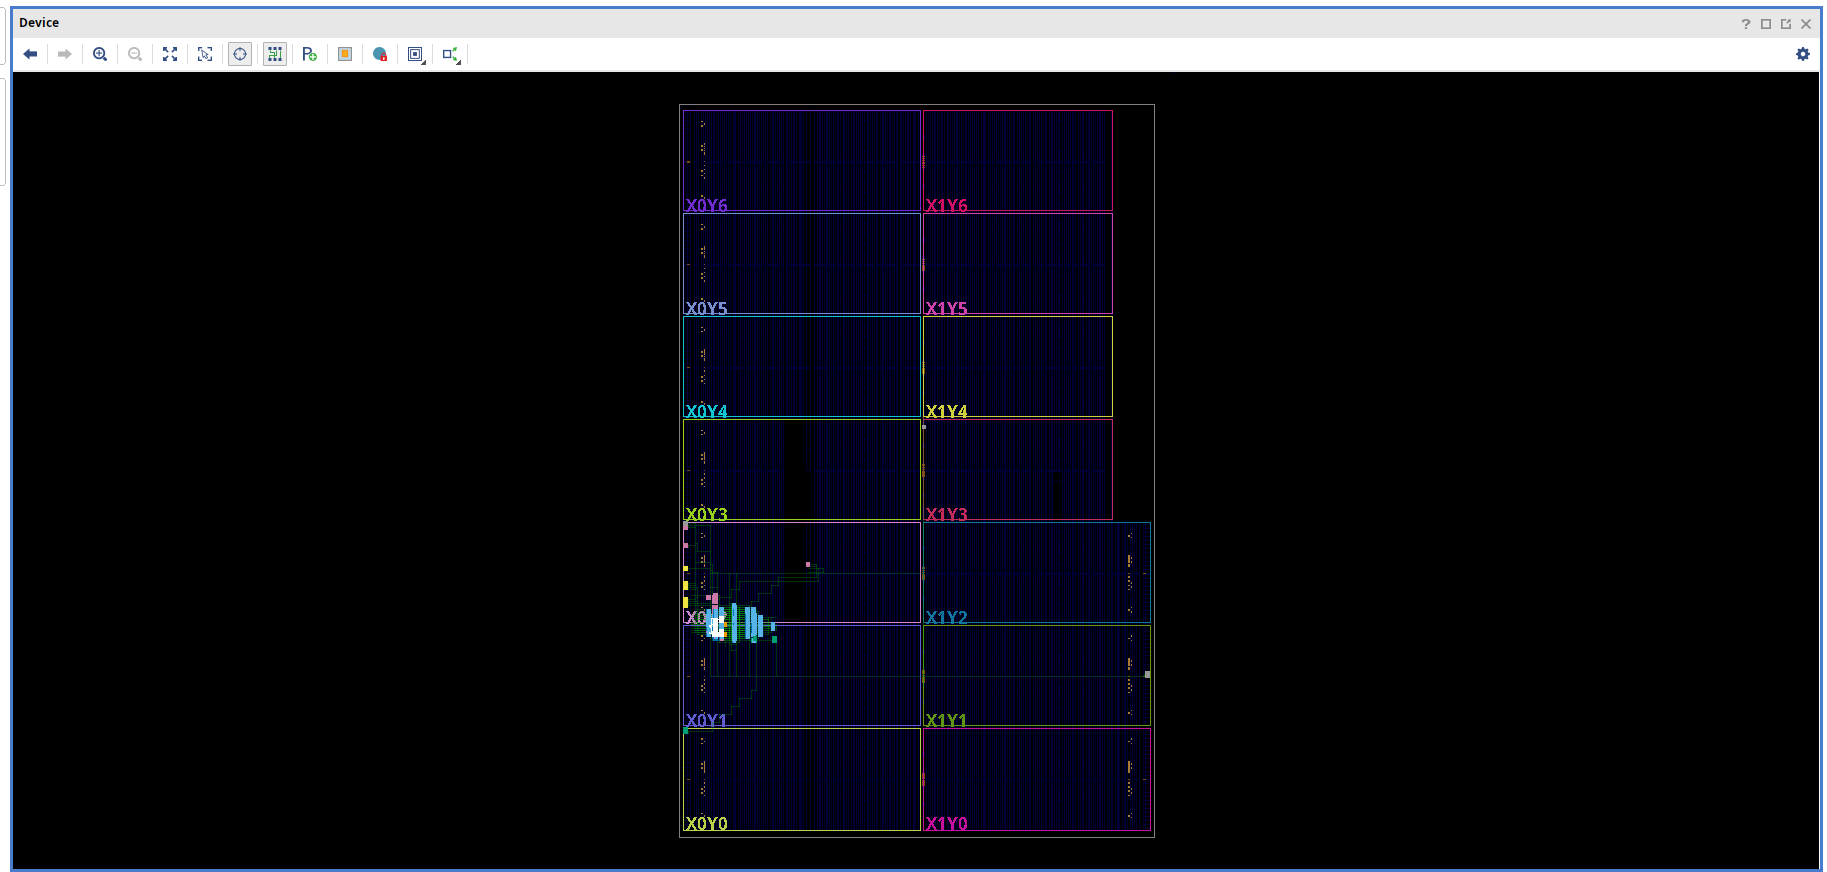
\includegraphics[width=\textwidth]{figures/vivado_device_1_whole}
    \caption{The whole device, its 14 clock regions outlined and named. The design is the
      coloured patch at the left edge of the lower half.}
  \end{subfigure}\hfill
  \begin{subfigure}[t]{0.49\textwidth}
    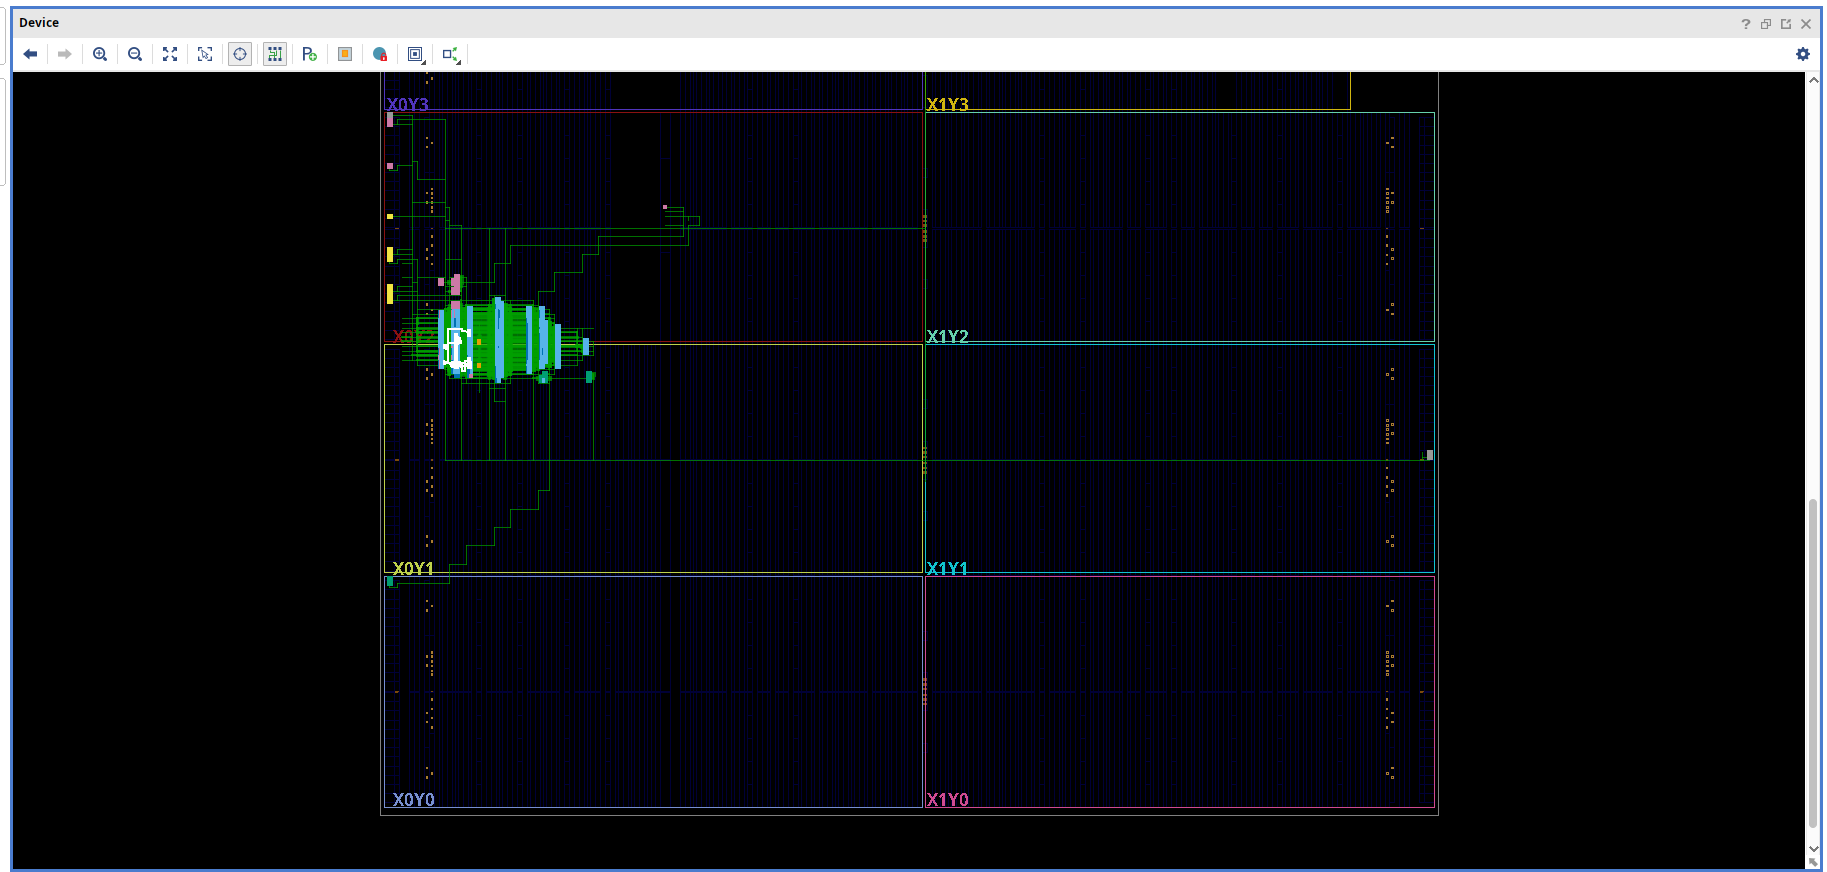
\includegraphics[width=\textwidth]{figures/vivado_device_2_regions}
    \caption{The lower clock regions. Vivado draws the routed nets in green; some run from
      the design out to the left and right edges of the device.}
  \end{subfigure}
  \par\medskip
  \begin{subfigure}[t]{0.49\textwidth}
    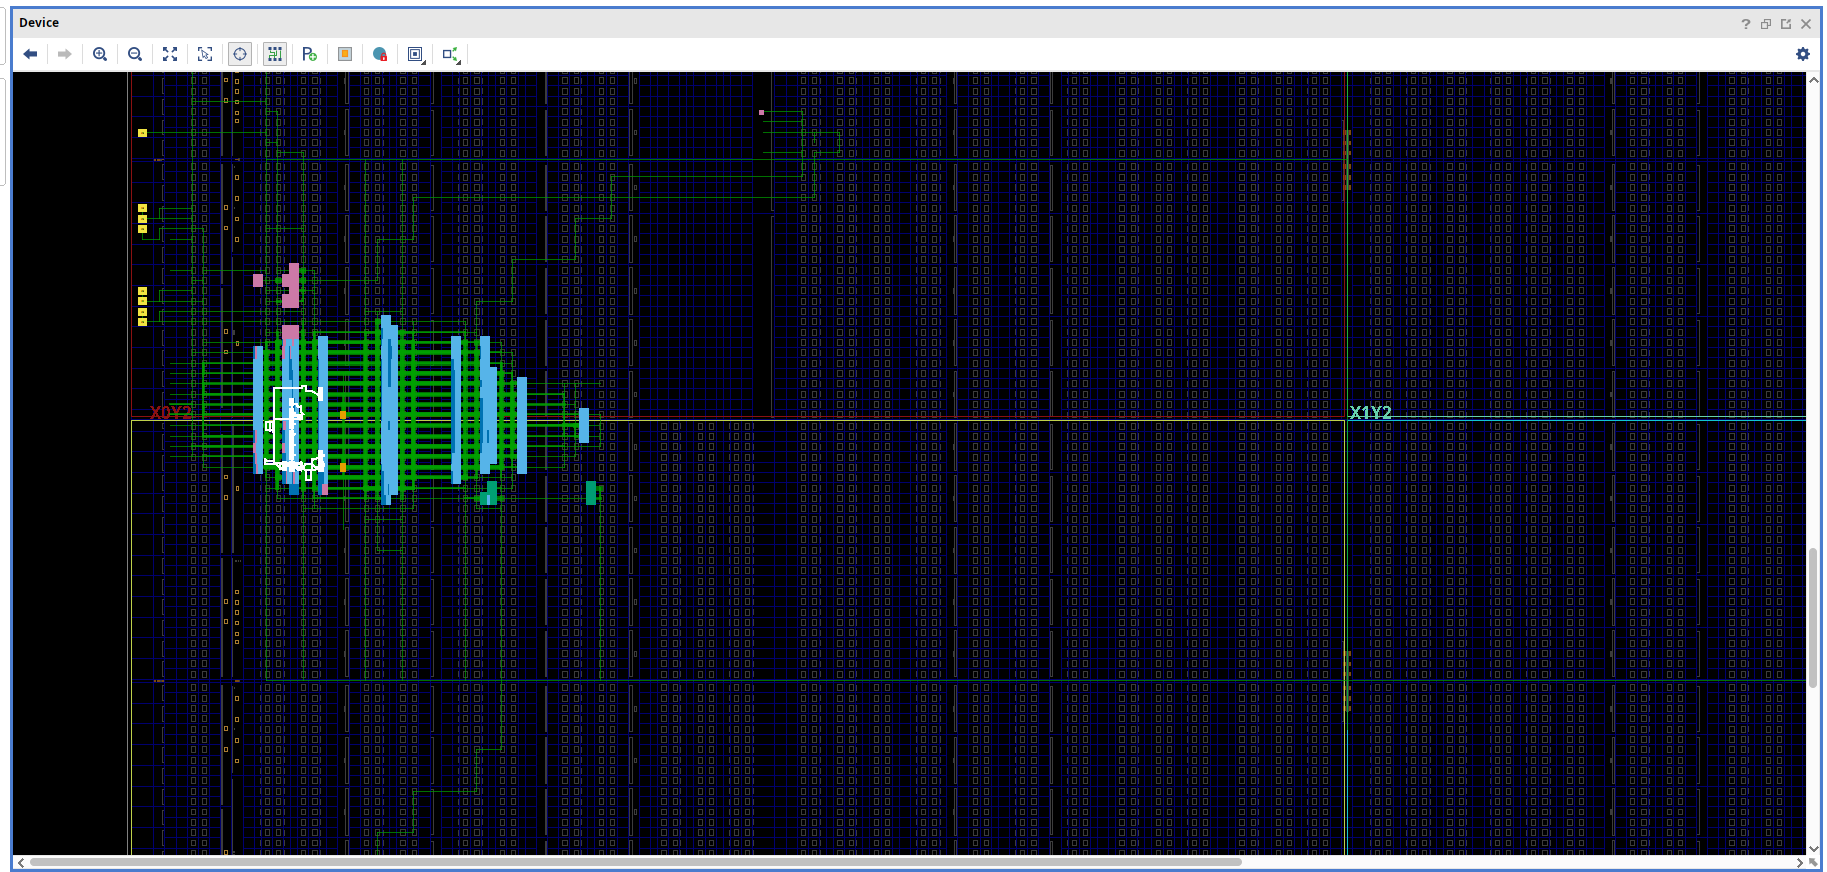
\includegraphics[width=\textwidth]{figures/vivado_device_3_design}
    \caption{The design: the register file and the rest of the core in the middle, the LED
      outputs at the left edge, and the worst path in white.}
  \end{subfigure}\hfill
  \begin{subfigure}[t]{0.49\textwidth}
    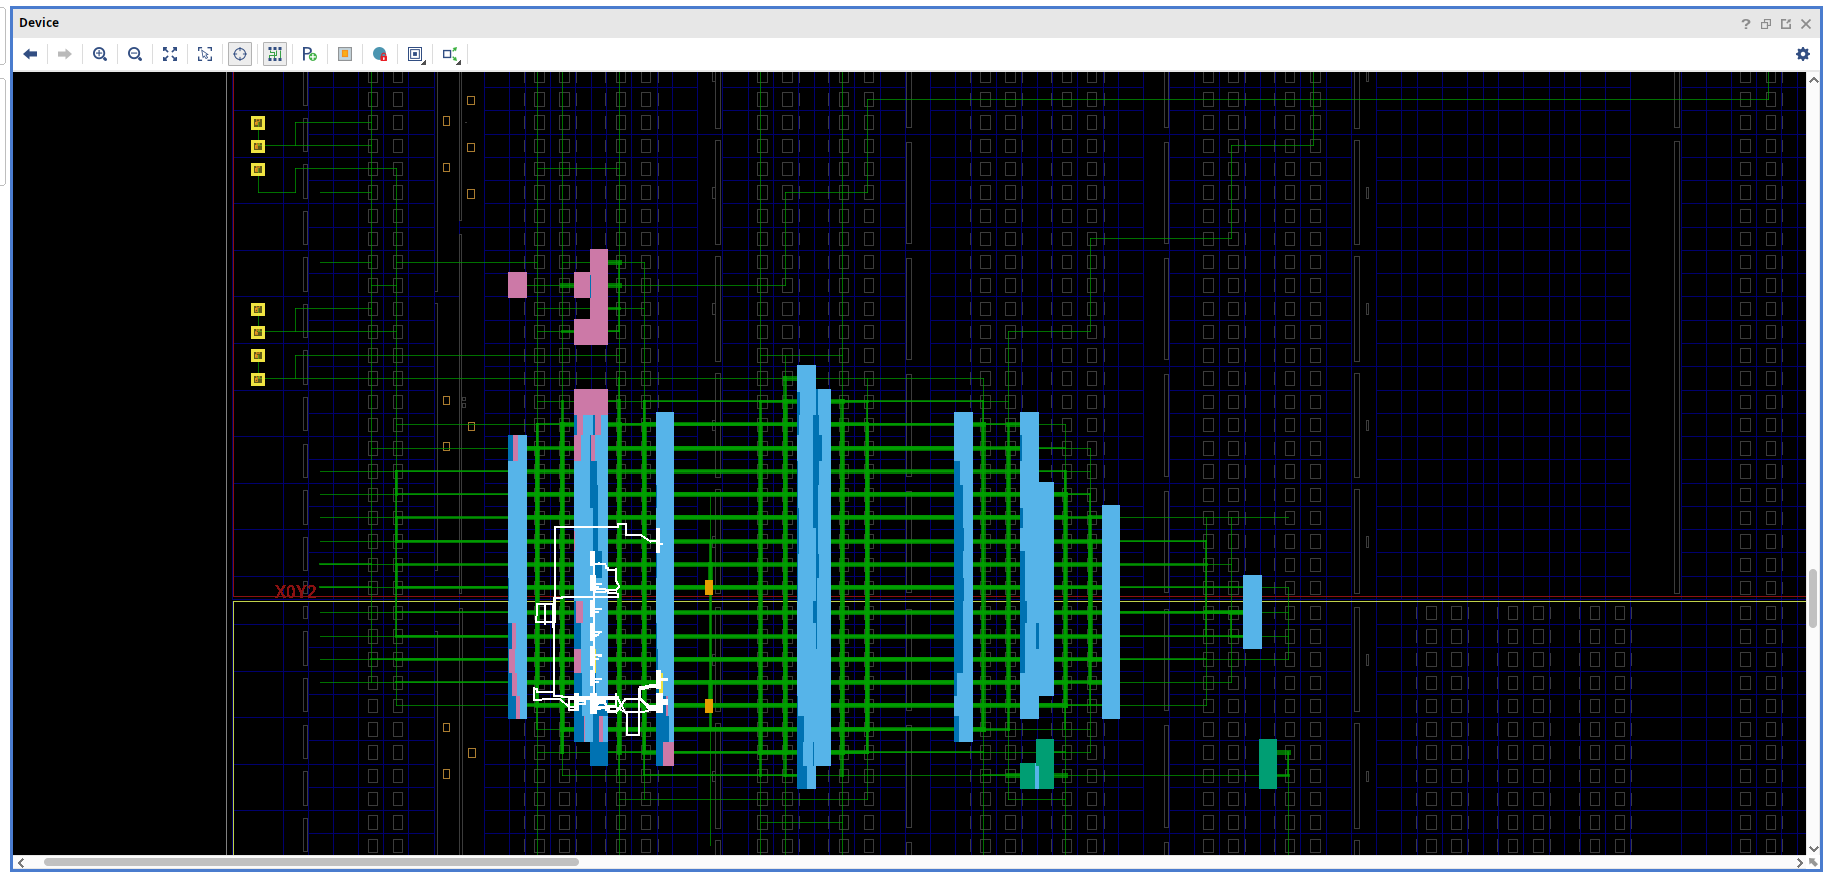
\includegraphics[width=\textwidth]{figures/vivado_device_4_path}
    \caption{Around the worst path, which ends at a write port of the register file's LUT
      RAM.}
  \end{subfigure}
  \caption{Vivado's Device view of the routed design, zoomed in from the whole device to the
    worst setup path. The modules are in their colours (Table~\ref{tab:module-colours}) and
    the worst path is selected; Routing Resources is on.}
  \label{fig:device-zoom}
\end{figure}

\begin{figure}[htbp]
  \centering
  \begin{subfigure}{\textwidth}
    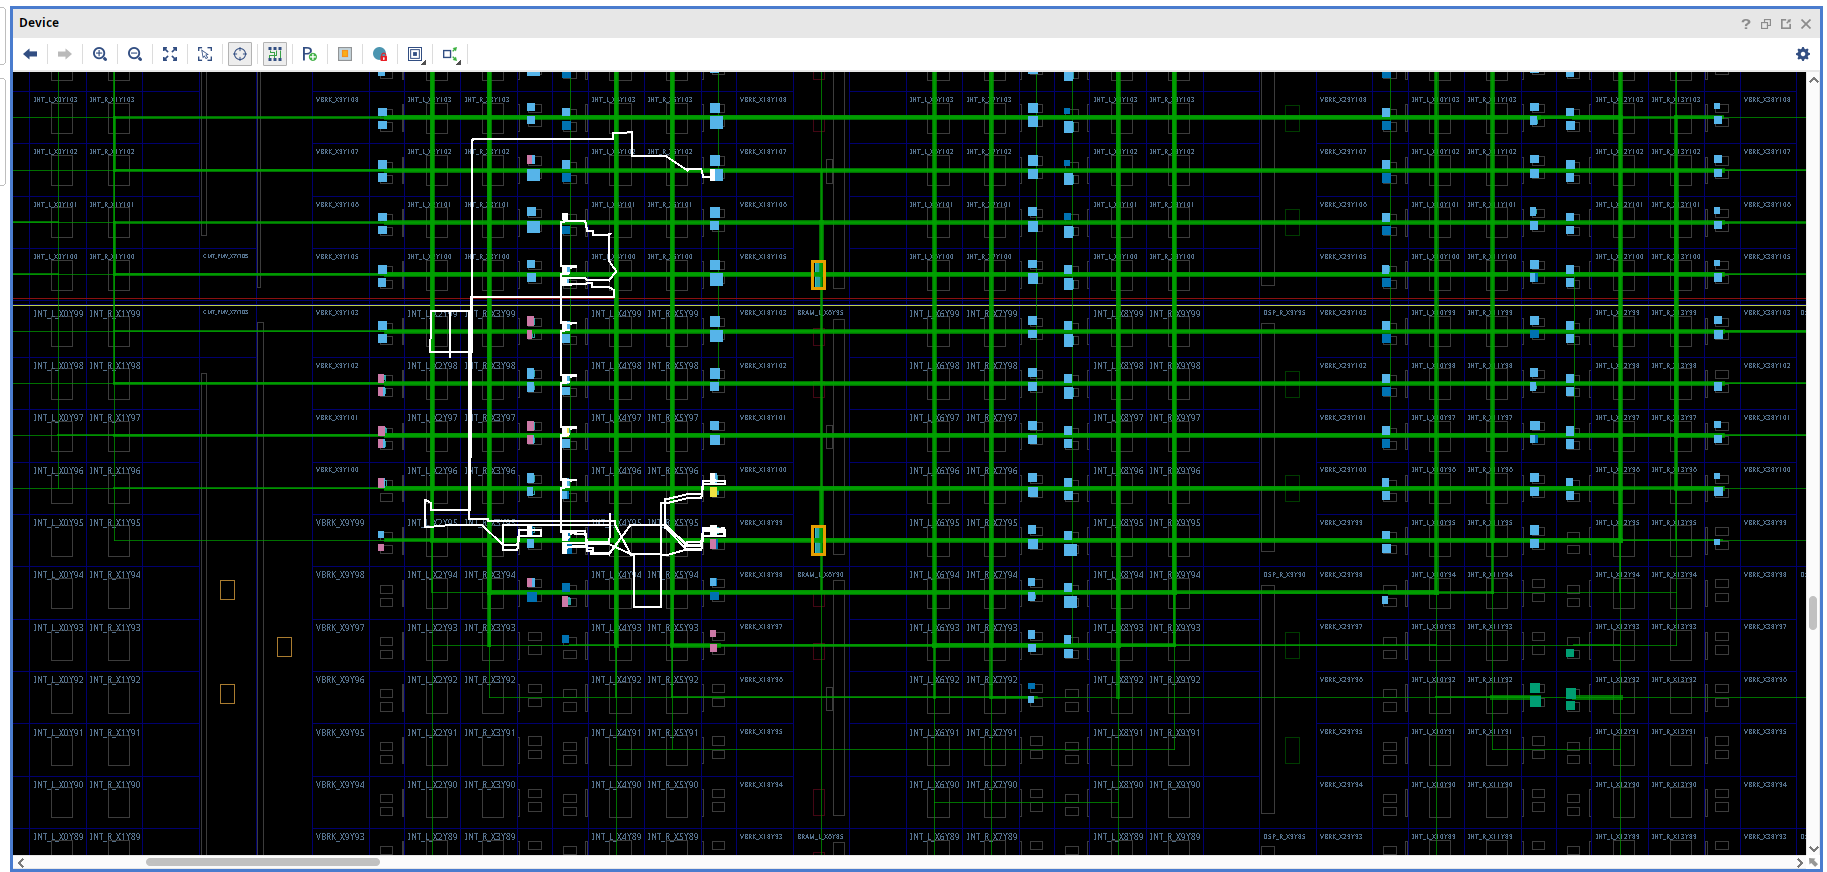
\includegraphics[width=\textwidth]{figures/vivado_device_5_routing_on}
    \caption{Routing Resources on, its toolbar button pressed: each of the path's nets follows
      the wires the router chose through the interconnect tiles (\texttt{INT\_L},
      \texttt{INT\_R}).}
  \end{subfigure}
  \par\medskip
  \begin{subfigure}{\textwidth}
    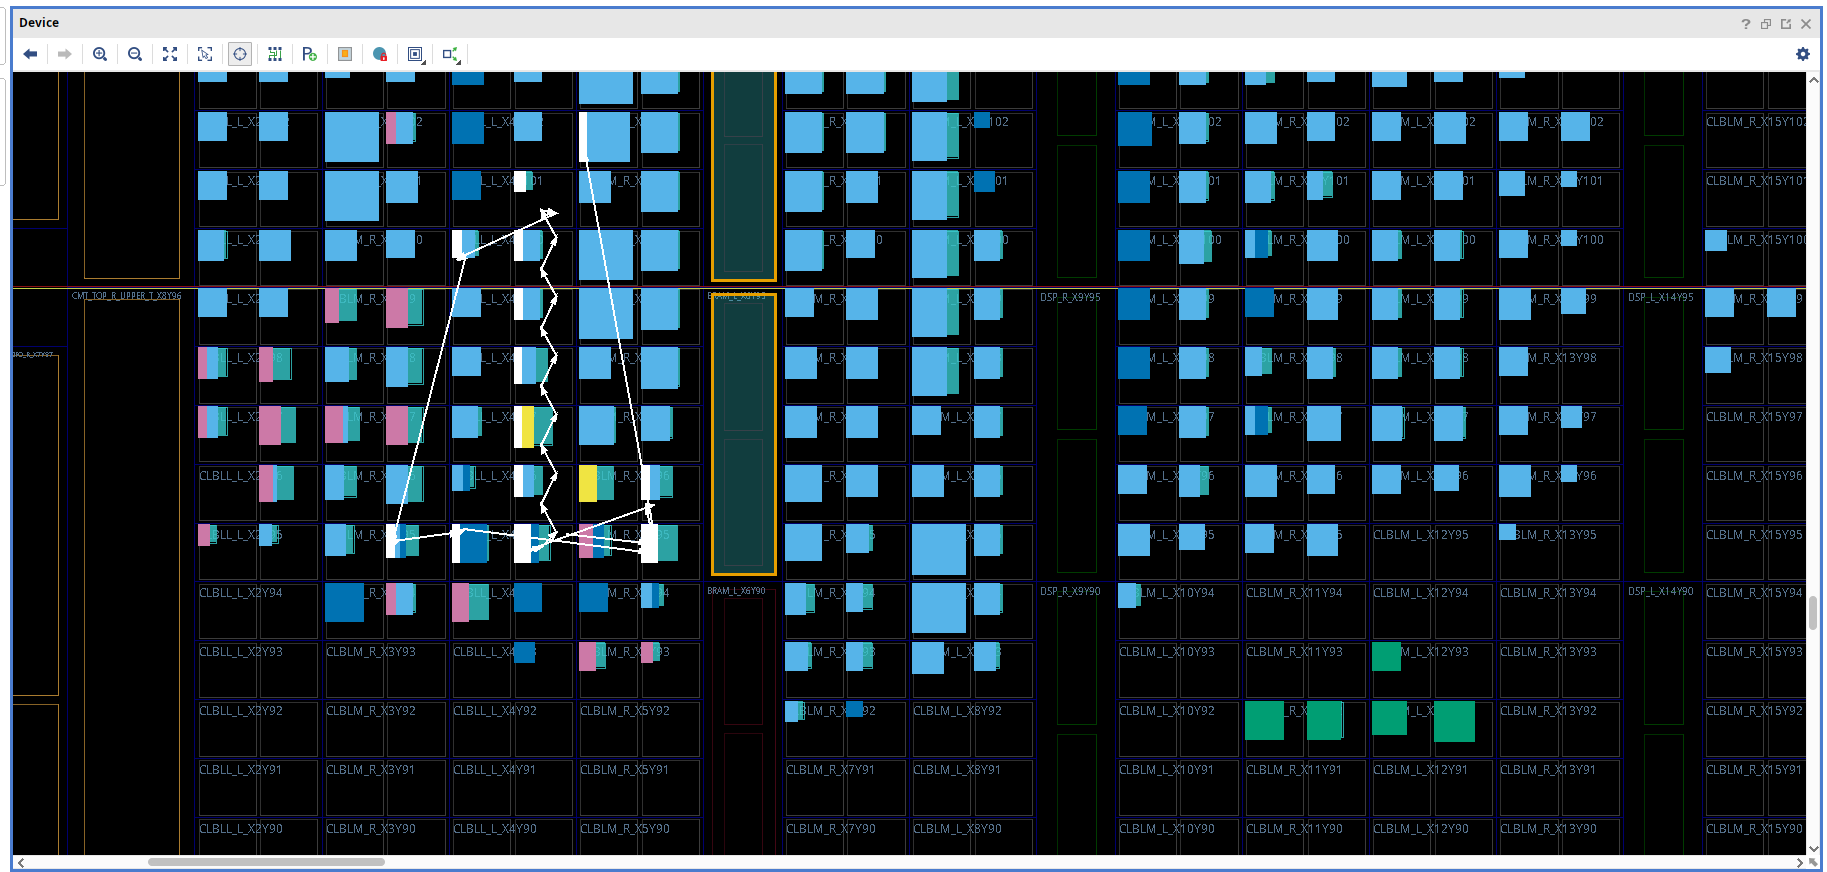
\includegraphics[width=\textwidth]{figures/vivado_device_6_routing_off}
    \caption{Routing Resources off, zoomed further in: each net is drawn as a straight line
      from its driver to its load, over the slices (\texttt{CLBLL}, \texttt{CLBLM}) that hold
      the path's cells.}
  \end{subfigure}
  \caption{The worst setup path, from \texttt{cpu/instr\_reg[3]} to the register-file write:
    15 logic levels and 0.219~ns of slack at 200~MHz, selected in white.}
  \label{fig:worst-path}
\end{figure}

\chapter{Results on the board}
\label{ch:board}

Everything in this chapter was captured from the real board. Each demo's bitstream is loaded
into the FPGA over JTAG and never written to the flash, which keeps Digilent's factory
bitstream at offset~0: the board boots its demo again at the next power-on. Flash boot writes
only the program, at the flash's code offset, over part of the factory demo's data. From the
moment the bitstream starts to load, the host records the UART at 115\,200~baud, 8N1, with a
timestamp on every read, accurate to about 2~ms. The raw captures are committed in
\texttt{docs/design/captures/}, and \texttt{make figures} renders the figures below from them;
\texttt{docs/design/figures/README.md} gives the procedure.

\section{Mandelbrot in BRAM boot}

The mandelbrot demo is the committed firmware image, the one the golden trace was simulated
with. Its bitstream is the synthesised design with \texttt{BOOT\_ADDR} set to
\texttt{BOOT\_ADDR\_BRAM}, as the testbench sets it, so the core starts from the image in the
RAM as soon as configuration ends. Figure~\ref{fig:board-mandelbrot} shows the first frame
the board sent.

\begin{figure}[htbp]
  \centering
  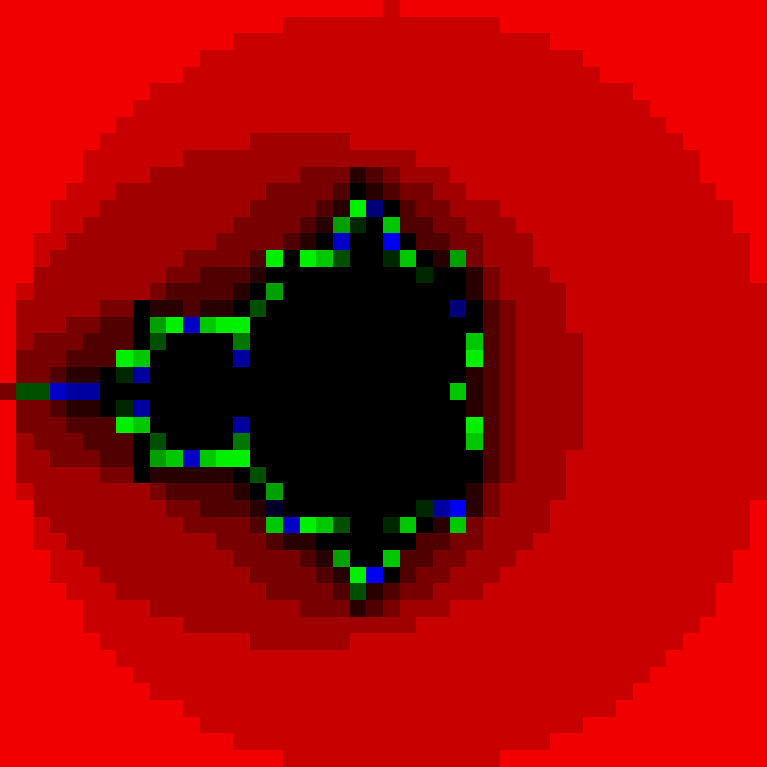
\includegraphics[width=0.6\textwidth]{figures/board_mandelbrot}
  \caption{The mandelbrot demo's first frame, rendered from the board's UART capture as a
    terminal shows it: 46 rows of 46 pixels, each pixel two spaces on a 24-bit background
    colour.}
  \label{fig:board-mandelbrot}
\end{figure}

\paragraph{The board against the simulation.} The first frame the board sent is 11\,014
bytes long, and it is byte for byte the UART bytes of the golden trace. The golden trace is in
turn byte for byte what \texttt{fw/mandelbrot.c} prints when compiled natively
(\texttt{docs/baseline.md}), so the board, the simulation and the C source agree.

\paragraph{Frame time.} On the board the frame took 1031.8~ms, from its first byte to the
first byte of the next frame. The simulation took 206\,292\,808 cycles from reset to the start
of the next frame, 1031.46~ms at 200~MHz. The start-up code before the first byte is a few
dozen instructions, so the two measure the same interval. They agree to 0.3~ms, within the
timestamps' accuracy of about 2~ms, or 0.2\,\%: to that accuracy, the board takes the cycles
the simulation counts, at 200~MHz. Most
of the frame is the UART. At ten bits per byte, sending the 11\,014 bytes takes about
956~ms, and \texttt{putchar} waits for each byte to leave before it returns, so the
computation itself takes about 75~ms.

\section{riscv\_logo}

The riscv\_logo demo rotates and zooms the RISC-V logo, a 16 by 16 bitmap, tiled over a grid
of 40 by 40 pixels in the 16 standard terminal colours, here in xterm's palette. One turn is
64 frames. The board sent them in 35.3~s, 551~ms a frame on average and 388 to 675~ms each:
a frame is 4\,400 to 7\,700 bytes, and the UART sets the pace, as for mandelbrot.
Figure~\ref{fig:board-riscv-logo} shows every eighth frame, and
Figure~\ref{fig:board-riscv-logo-animated} the whole turn. The 72 frames captured are, byte
for byte, what \texttt{fw/riscv\_logo.c} prints when compiled natively: no byte was lost on
the way to the host.

\begin{figure}[htbp]
  \centering
  \foreach \frame in {1,9,...,57} {%
    \includegraphics[page=\frame, width=0.118\textwidth]{figures/board_riscv_logo}\hfill}%
  \unskip
  \par\medskip
  \begin{minipage}[c]{0.8\textwidth}
    \caption{The riscv\_logo demo on the board: frames 0, 8, \ldots, 56 of one turn, left to
      right, 45 degrees apart, rendered from the UART capture. The animation plays in the
      repository's README, at
      \url{https://github.com/amitmalach/FPGA_RiscV_MultiCycle\#running-the-demos},
      the address the code on the right holds.}
    \label{fig:board-riscv-logo}
  \end{minipage}\hfill
  \begin{minipage}[c]{0.15\textwidth}
    \raggedleft
    \qrcode[height=2cm]{https://github.com/amitmalach/FPGA_RiscV_MultiCycle\#running-the-demos}
  \end{minipage}
\end{figure}

\begin{figure}[htbp]
  \centering
  \animategraphics[width=0.5\textwidth, autoplay, loop, controls]{1.81}%
    {figures/board_riscv_logo}{}{}
  \caption{The riscv\_logo demo's turn, all 64 frames, at the board's average rate of 1.81
    frames per second. Only Adobe Reader plays the animation; other viewers show the first
    frame.}
  \label{fig:board-riscv-logo-animated}
\end{figure}

\section{tinyraytracer in flash boot}

tinyraytracer is 29\,016 bytes of code and constants, almost five times the 6~KB RAM, so it
runs only in flash boot, executed in place from the flash (Chapter~\ref{ch:flash}). Its flash
image was written to the code window at \texttt{0xD00000} with ``Configuration File Only''. A
readback of the whole 32~MB chip afterwards differed from the one taken before only in the
image's own 29\,016 bytes: the factory bitstream at offset~0 was not touched. Before each
capture, the capture script reads the code window back and compares it with the binary.

\paragraph{The reset button.} With the flash-boot bitstream loaded over JTAG, the core printed
nothing and the LEDs stayed dark: in the capture behind Figure~\ref{fig:board-tinyraytracer},
no byte arrived in the 44~s between the end of the load and a press of the CPU reset button.
From the press on, the demo ran to the end, so flash boot works on this board with the reset
button pressed once after each load. Everything points to the core losing its first fetch
from the flash straight after configuration: that fetch is \texttt{li gp, IO\_BASE}, the first
instruction of \texttt{fw/start\_spiflash.S}, and without it the UART writes go to RAM
address~8, over the code that start-up has just copied there. Two parts of the design can
lose it. \texttt{STARTUPE2} hands the CCLK pin to user logic only after a few cycles of
\texttt{USRCCLKO}, as Vivado's simulation model of the primitive shows, so the first SPI
transaction can miss its first clock edges; and \texttt{IOBus} drops a flash read requested
before end of startup instead of stalling it, while the core starts fetching as soon as
configuration releases the flip-flops. The pitfall and its fix belong to
Chapter~\ref{ch:next}.

\paragraph{The Quad Enable bit.} Writing the image cost the board its power-on boot. The
write, with Vivado's \texttt{hw\_cfgmem} property \texttt{PROGRAM.SKIP\_QE\_BIT\_ERASE} at its
default, cleared the flash's non-volatile Quad Enable bit (S25FL256S configuration register~1,
bit~1), and a second write of the image with an SPIx4 \texttt{.prm} did not set it back. The
factory bitstream reads the flash four bits wide (opcode
\texttt{0x6C} in its BSPI register) and needs the bit: at the next power-on the FPGA stalled in
configuration, DONE low and no error flag set, with every byte of the flash intact. Vivado's
Tcl reads no flash register, so a small design of its own,
\texttt{docs/design/scripts/flashregs/FlashRegs.v}, loaded over JTAG, read the register
(\texttt{0x00}: the bit clear), wrote it back to \texttt{0x02}, and the FPGA configured from
the flash again over JTAG, DONE high; a further write of the image with the property set kept
the bit, and at the next power-on the board booted Digilent's factory demo again. This pitfall
belongs to Chapter~\ref{ch:next} too.

\paragraph{The picture.} Figure~\ref{fig:board-tinyraytracer} shows what the board sent:
48 by 24 pixels, each one terminal cell, a space on one of xterm's 256 colours.
The run is 21\,412 bytes long and is, byte for byte, what \texttt{fw/tinyraytracer.c} prints
when compiled natively, with \texttt{libm} and floating point in software on the board and in
the host's hardware on the PC. The picture took 126.8~s, 110~ms a pixel: every
floating-point operation is a call into \texttt{libgcc}, and every instruction outside the RAM
is fetched from the flash, one SPI transaction each.

\begin{figure}[htbp]
  \centering
  
\includegraphics[width=0.45\textwidth]{figures/board_tinyraytracer}
  \caption{tinyraytracer in flash boot, rendered from the board's UART capture: four spheres,
    of ivory, glass, red rubber and mirror, over a chequered floor and lit by three lights, at
    48 by 24 terminal cells.}
  \label{fig:board-tinyraytracer}
\end{figure}

\section{ST\_NICCC}

ST\_NICCC was not run. It needs the 640~KB scene data at \texttt{0xC00000} and its own
program in the code window, two more writes over the factory demo's data, and the reset
button as above.

\section{blinker and sieve}

Both ran in BRAM boot. The blinker alternates LEDs 0 and 2 with LEDs 1 and 3 every 5.24~ms
in simulation, about 95 times a second: too fast to see, and on the board LD0 to LD3 glowed
steadily at about half brightness while LD4 to LD7 stayed dark. sieve printed the 31 primes
below 128 and its checksum, \texttt{1772A48F OK}, every 96~ms; the 59 rounds captured are,
byte for byte, what \texttt{fw/sieve.c} prints when compiled natively, but for the checksum's
hex digits, which \texttt{fw/print.c} prints in upper case.

\chapter{For the next student}
\label{ch:next}
\planned{the pitfalls checklist (symptom, cause, where it is handled) and a ranked list of
extensions.}

\chapter{Conclusions}
\planned{what was built, what it shows, and what is left.}

\appendix

\chapter{Memory map}
\planned{the full memory map, matching \texttt{rtl/defines.vh}.}

\chapter{Make targets}
\planned{every make target, what it runs and what it needs.}

\chapter{ISA coverage}
\label{app:isa}
\planned{the RV32I instructions the core executes, and what it leaves out.}

\begin{thebibliography}{9}
\raggedright  % long URLs do not break
\phantomsection\addcontentsline{toc}{chapter}{\bibname}

\bibitem{levy-learnfpga}
B.~Levy, \emph{learn-fpga}, ``From Blinker to RISC-V'', GitHub repository.
\url{https://github.com/BrunoLevy/learn-fpga}

\bibitem{riscv-isa}
A.~Waterman and K.~Asanovi\'c (eds.), \emph{The RISC-V Instruction Set Manual, Volume~I:
Unprivileged ISA}, document version 20191213, RISC-V Foundation.

\bibitem{digilent-genesys2-rm}
Digilent, \emph{Genesys~2 Reference Manual}.
\url{https://digilent.com/reference/programmable-logic/genesys-2/reference-manual}

\bibitem{digilent-genesys2-sch}
Digilent, \emph{Genesys~2 Schematic}, 22 pages, 2015.

\bibitem{ug470}
AMD Xilinx, \emph{7 Series FPGAs Configuration User Guide}, UG470.

\bibitem{ug835}
AMD Xilinx, \emph{Vivado Design Suite Tcl Command Reference Guide}, UG835.

\end{thebibliography}

\end{document}
